%------------------------------------------------------------------------------
\chapter{Control region distributions}
\label{sec:app}
%------------------------------------------------------------------------------
In this appendix, the distributions for all the kinematic and reconstructed variables from all the four control regions B, C, D and D1 are provided. 

In the control region, the other backgrounds are from the MC simulation and the multijet background is calculated from the equation below:

\begin{equation}
	N_{\text{j}}^{\text{Multijet}}[i] = N_{\text{j}}^{\text{Data}}[i] - N_{\text{j}}^{\text{Other bkg.}}[i] \,,
	\label{eqn:app}
\end{equation}
where $\text{j}\in\{\text{B, C, D, D1}\}$ and $i=$ bin.

Fig.\ \ref{fig:app:cr_b} shows all the six distributions from CR B. Fig.\ \ref{fig:app:cr_c} shows all the six distributions from CR C. Fig.\ \ref{fig:app:cr_d} shows all the six distributions from CR D. Fig.\ \ref{fig:app:cr_d1} shows all the six distributions from CR D1.

\begin{figure}[hbt!]
	\centering
	\graphicspath{{figs/appendix/CRB/}}
	\begin{subfigure}{.35\textwidth}
		\centering
		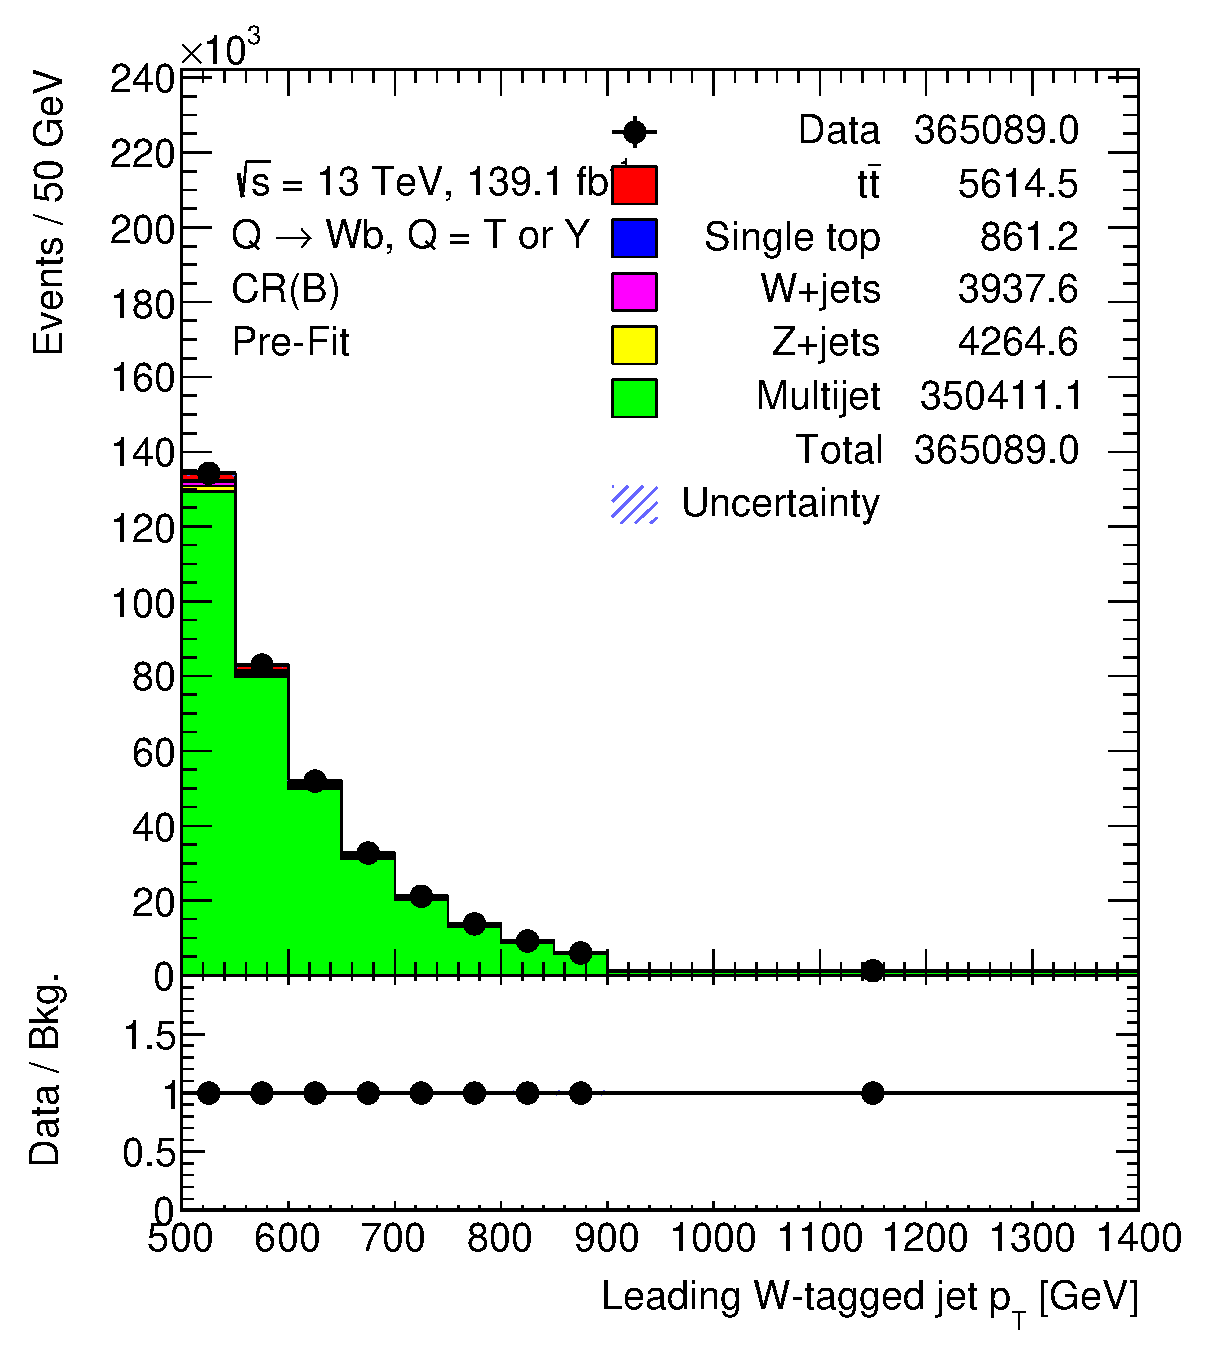
\includegraphics[width=\linewidth,height=\textheight,keepaspectratio]{CR_B_ljet_pt.eps}
		\caption{}
		\label{fig:app:cr_b:ljet_pt}
	\end{subfigure}\hspace{0.6cm}
	\begin{subfigure}{.35\textwidth}
		\centering
		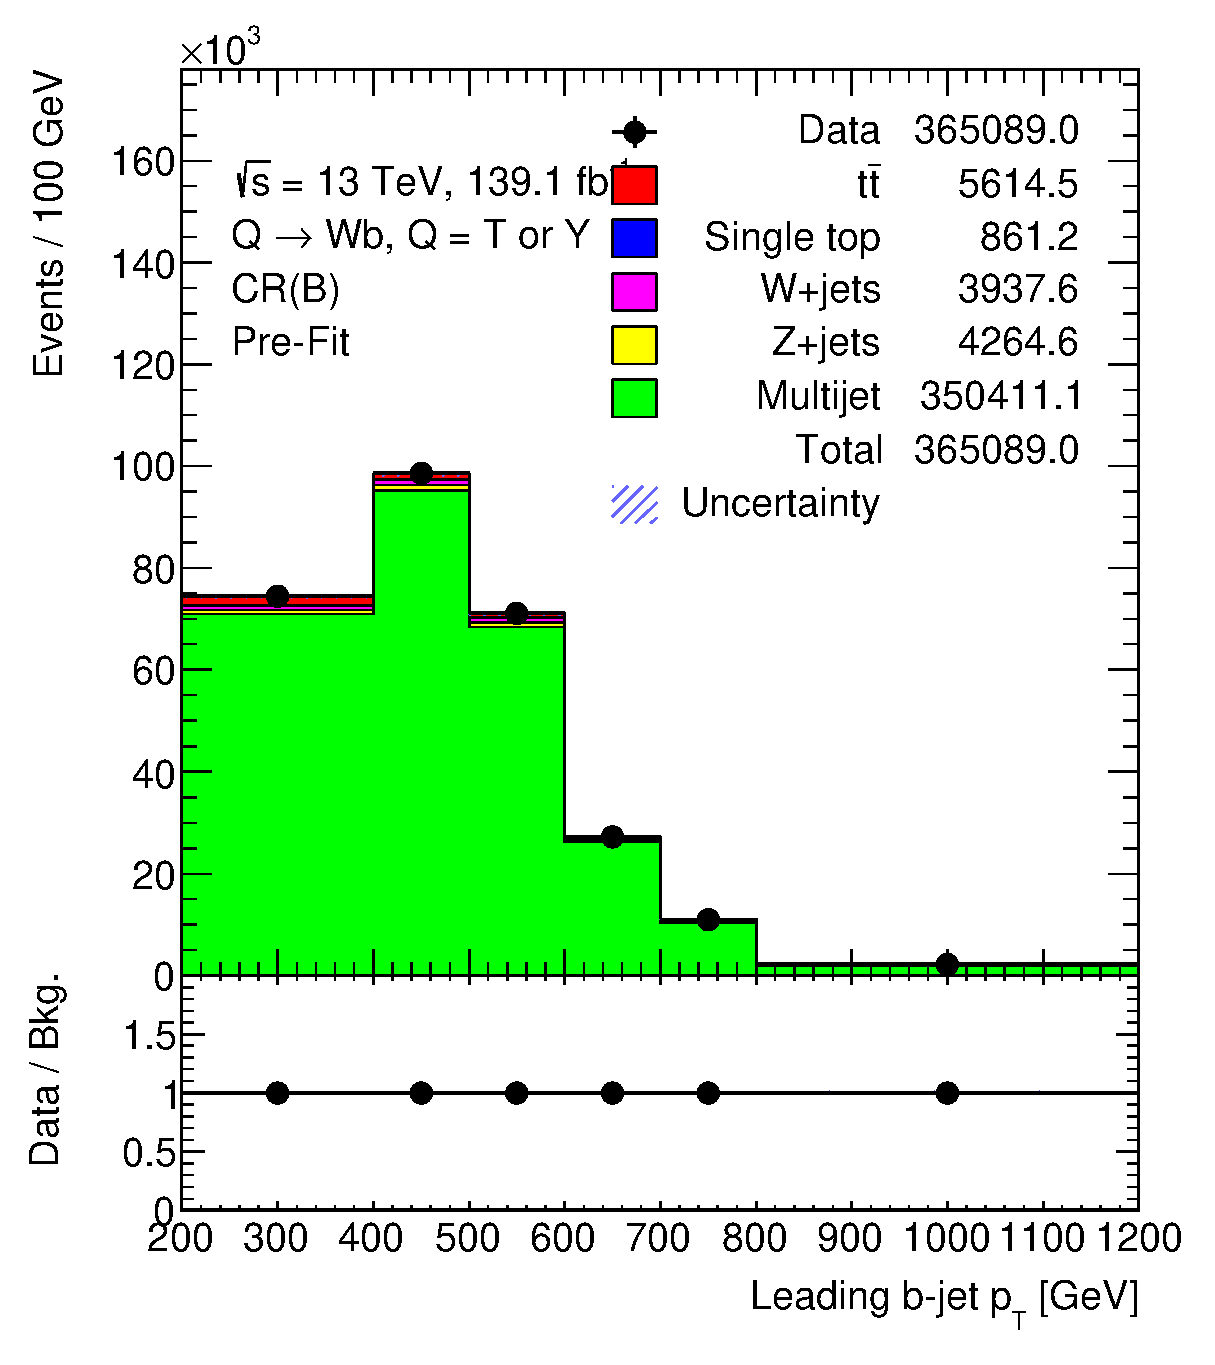
\includegraphics[width=\linewidth,height=\textheight,keepaspectratio]{CR_B_jet_pt.eps}
		\caption{}
		\label{fig:app:cr_b:jet_pt}
	\end{subfigure}
	\begin{subfigure}{.35\textwidth}
		\centering
		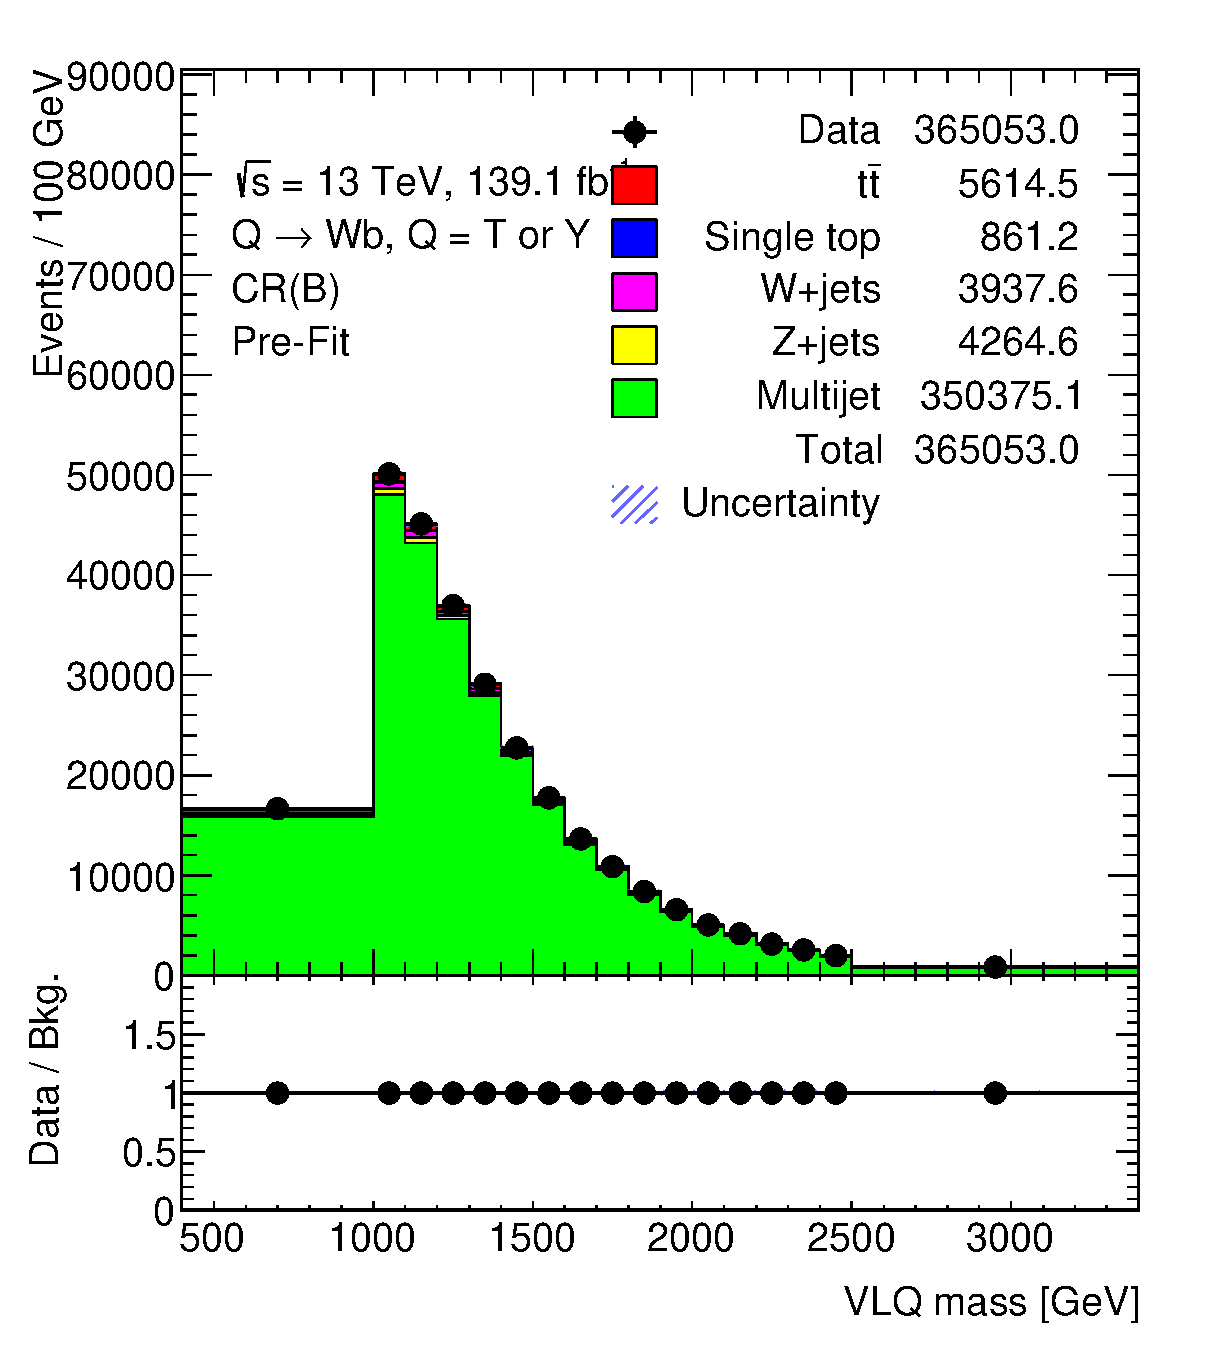
\includegraphics[width=\linewidth,height=\textheight,keepaspectratio]{CR_B_VLQM.eps}
		\caption{}
		\label{fig:app:cr_b:VLQM}
	\end{subfigure}\hspace{0.6cm}
	\begin{subfigure}{.35\textwidth}
		\centering
		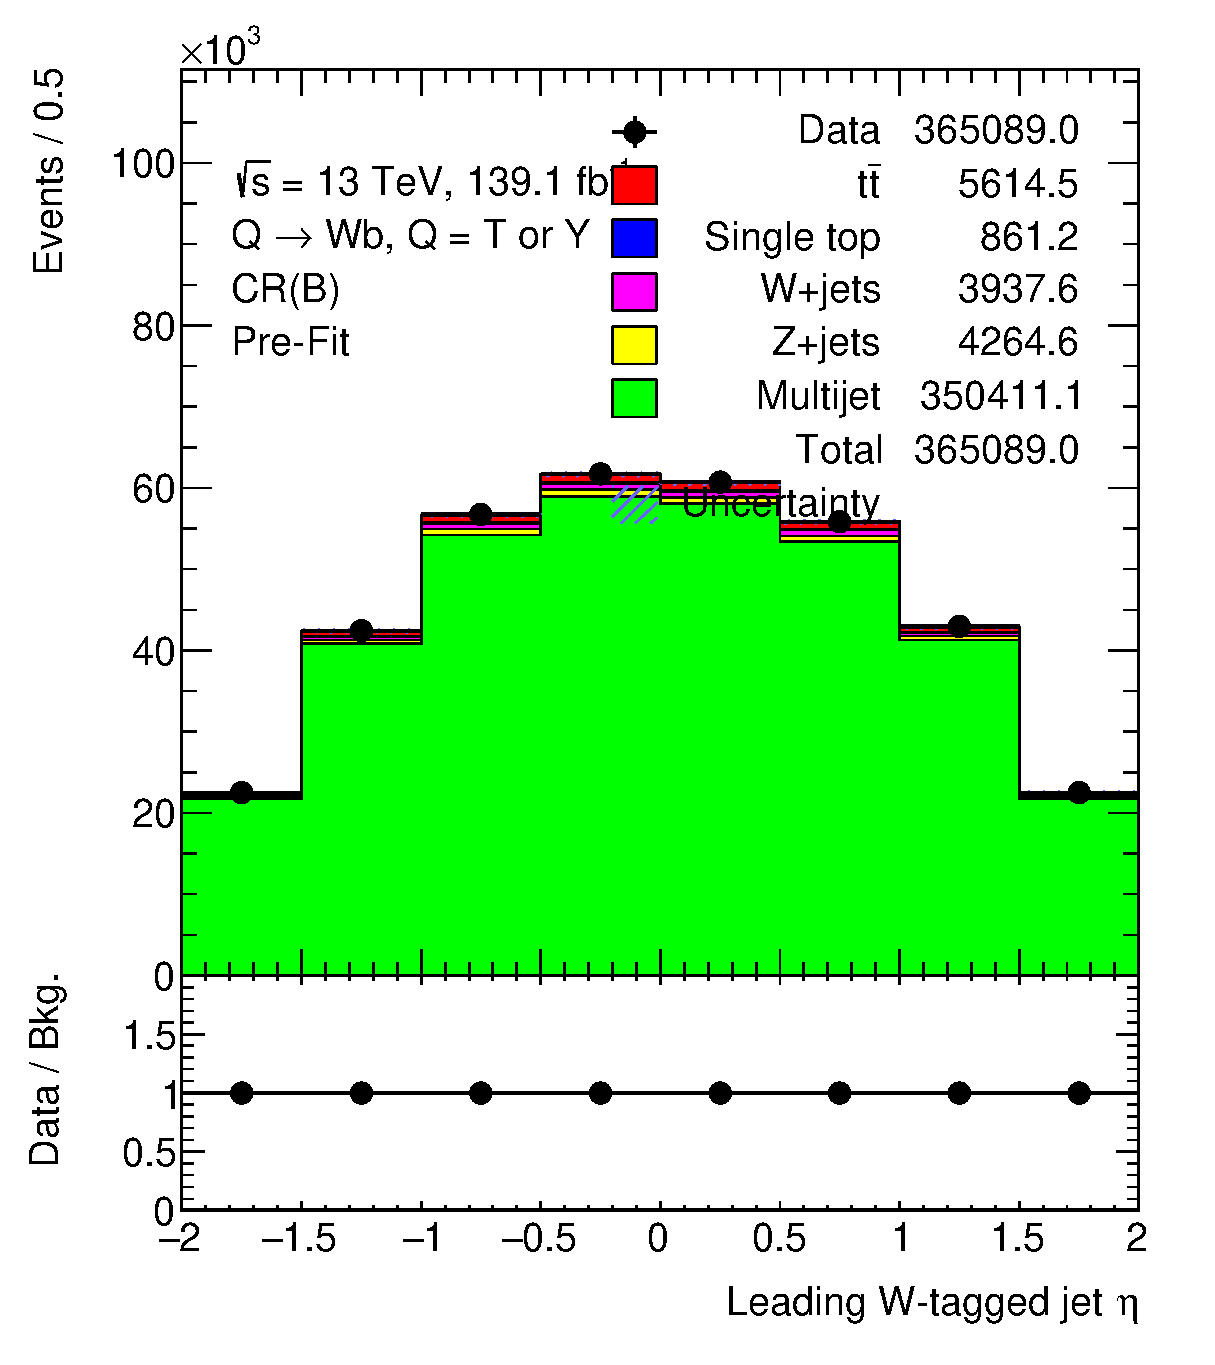
\includegraphics[width=\linewidth,height=\textheight,keepaspectratio]{CR_B_ljet_eta.eps}
		\caption{}
		\label{fig:app:cr_b:ljet_eta}
	\end{subfigure}
	\begin{subfigure}{.35\textwidth}
		\centering
		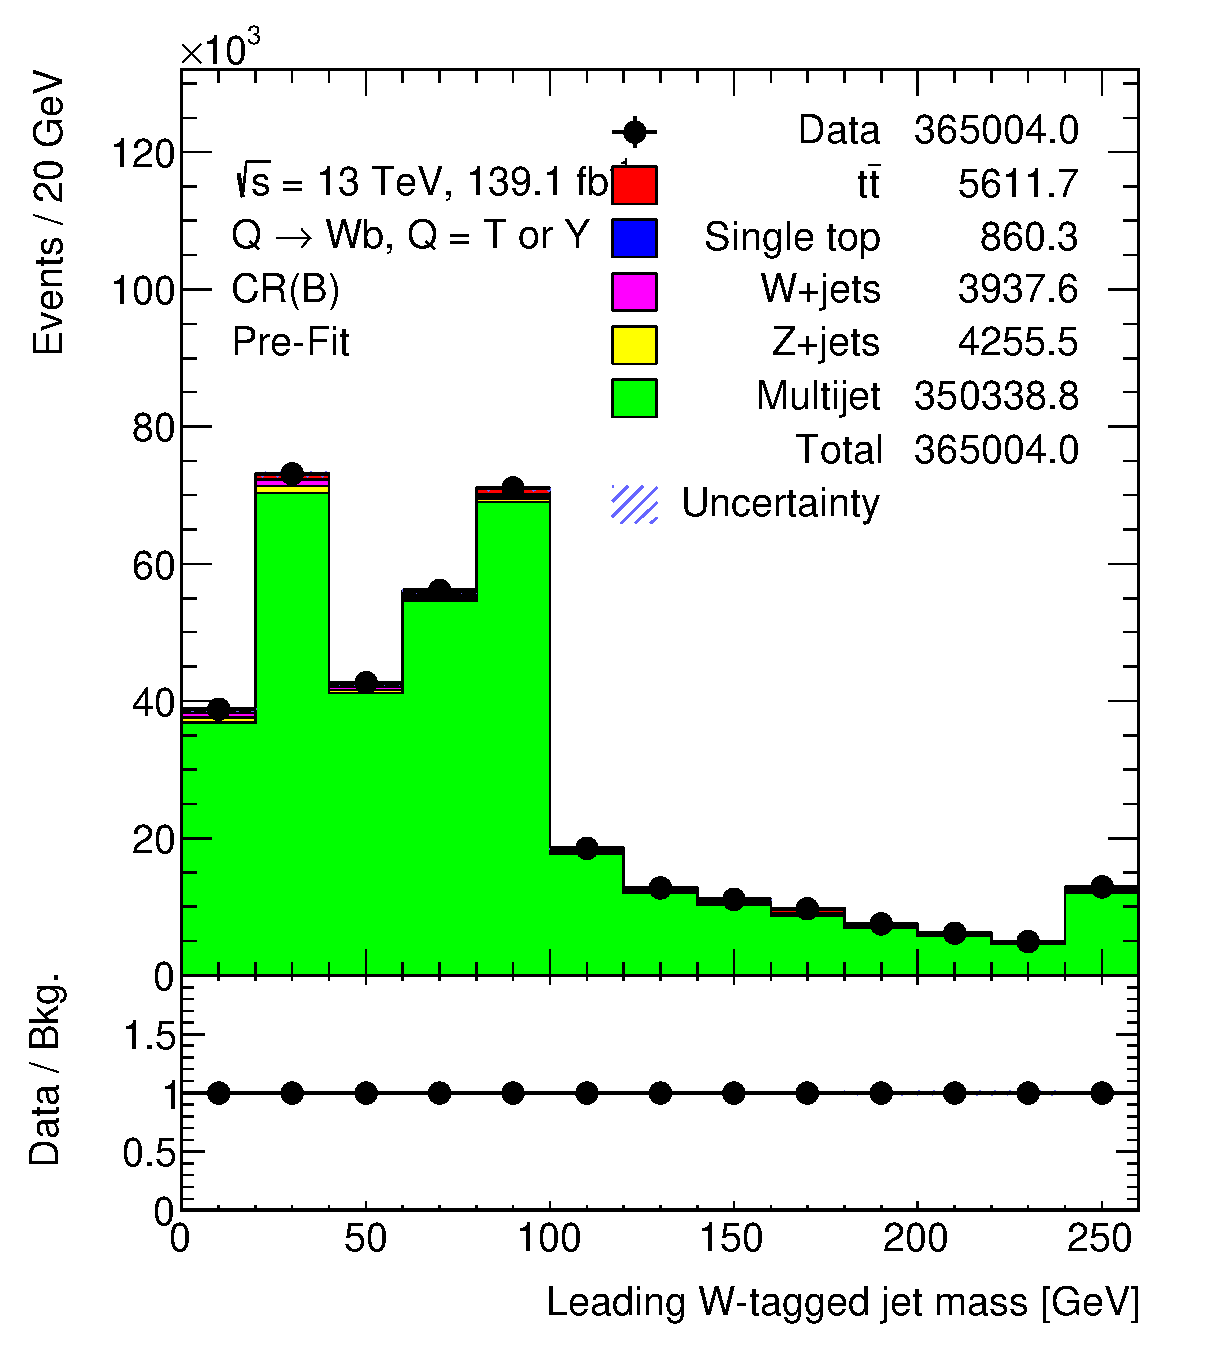
\includegraphics[width=\linewidth,height=\textheight,keepaspectratio]{CR_B_ljet_m.eps}
		\caption{}
		\label{fig:app:cr_b:ljet_m}
	\end{subfigure}\hspace{0.6cm}
	\begin{subfigure}{.35\textwidth}
		\centering
		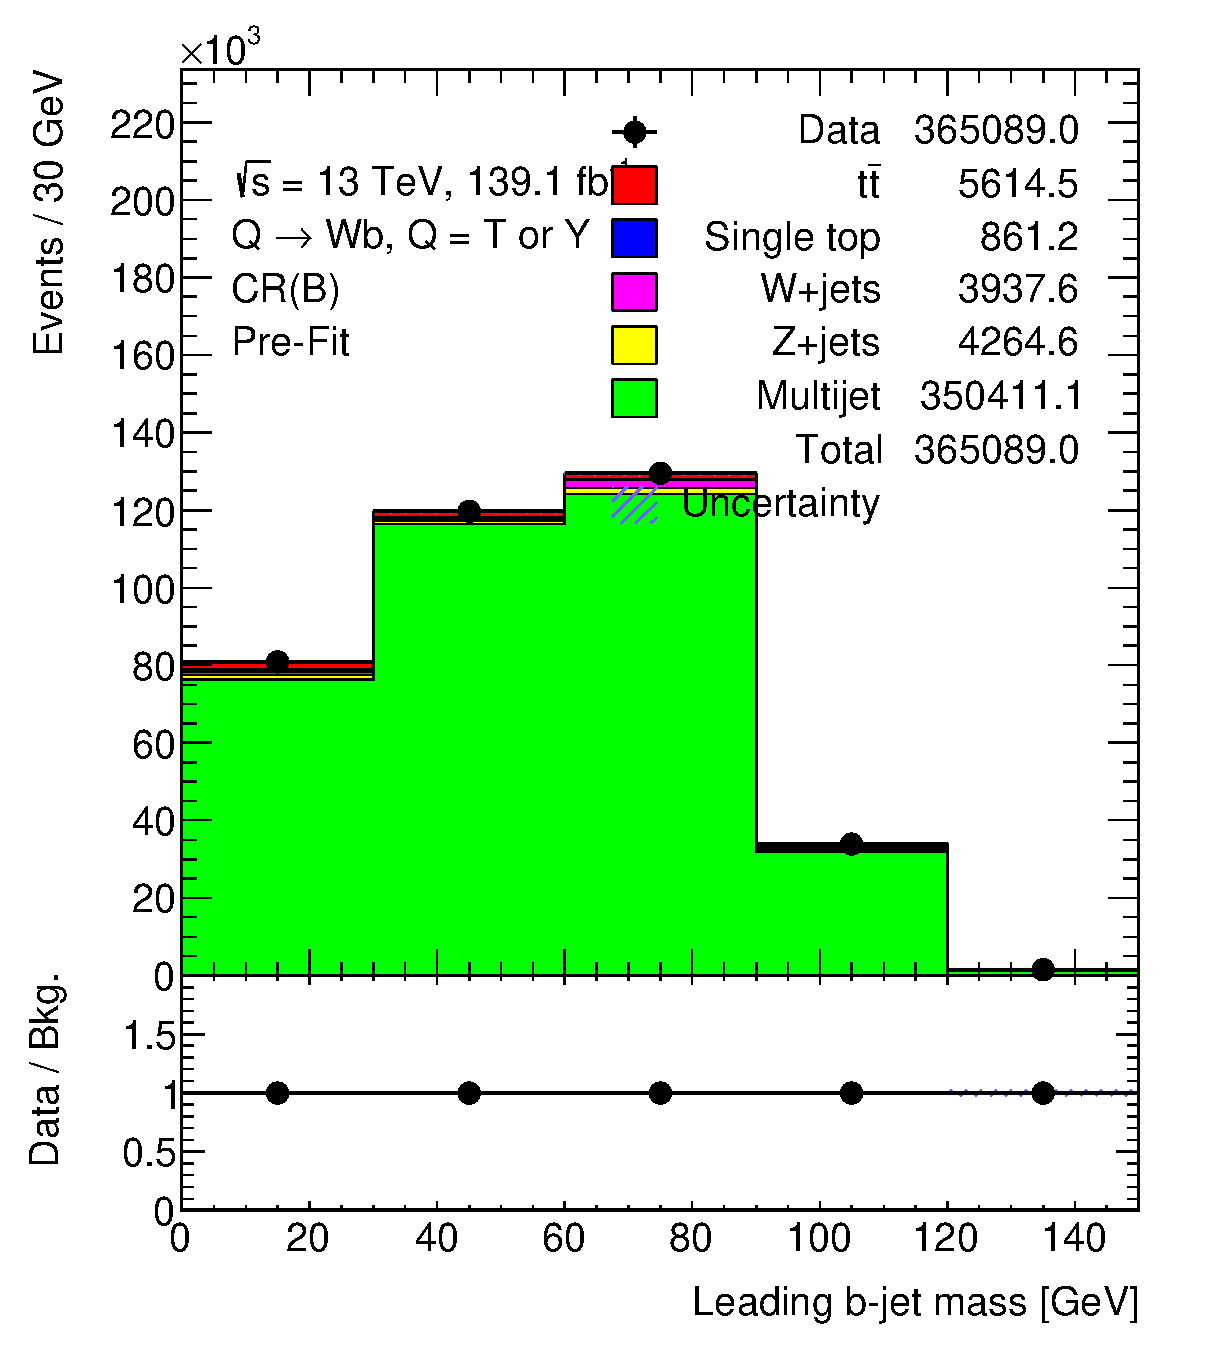
\includegraphics[width=\linewidth,height=\textheight,keepaspectratio]{CR_B_jet_m.eps}
		\caption{}
		\label{fig:app:cr_b:jet_m}
	\end{subfigure}
	\caption{A data/bkg.\ comparison of kinematic and reconstructed variables in CR B where the multijet background (in green) is calculated by Eqn.\ \ref{eqn:app} and the other backgrounds are from the MC simulation. The variables include (a) $p_{\text{T}}$ of $W$-tagged large-$R$ jet, (b) $p_{\text{T}}$ of leading $b$-tagged small-$R$ jet, (c) VLQ mass reconstructed from the kinematics of $W$-tagged large-$R$ jet and leading $b$-tagged small-$R$ jet, (d) $\eta$ distribution of $W$-tagged large-$R$ jet, (e) mass of $W$-tagged large-$R$ jet, and (f) mass of leading $b$-tagged small-$R$ jet.}
	\label{fig:app:cr_b}
\end{figure}







\begin{figure}[hbt!]
	\centering
	\graphicspath{{figs/appendix/CRC/}}
	\begin{subfigure}{.35\textwidth}
		\centering
		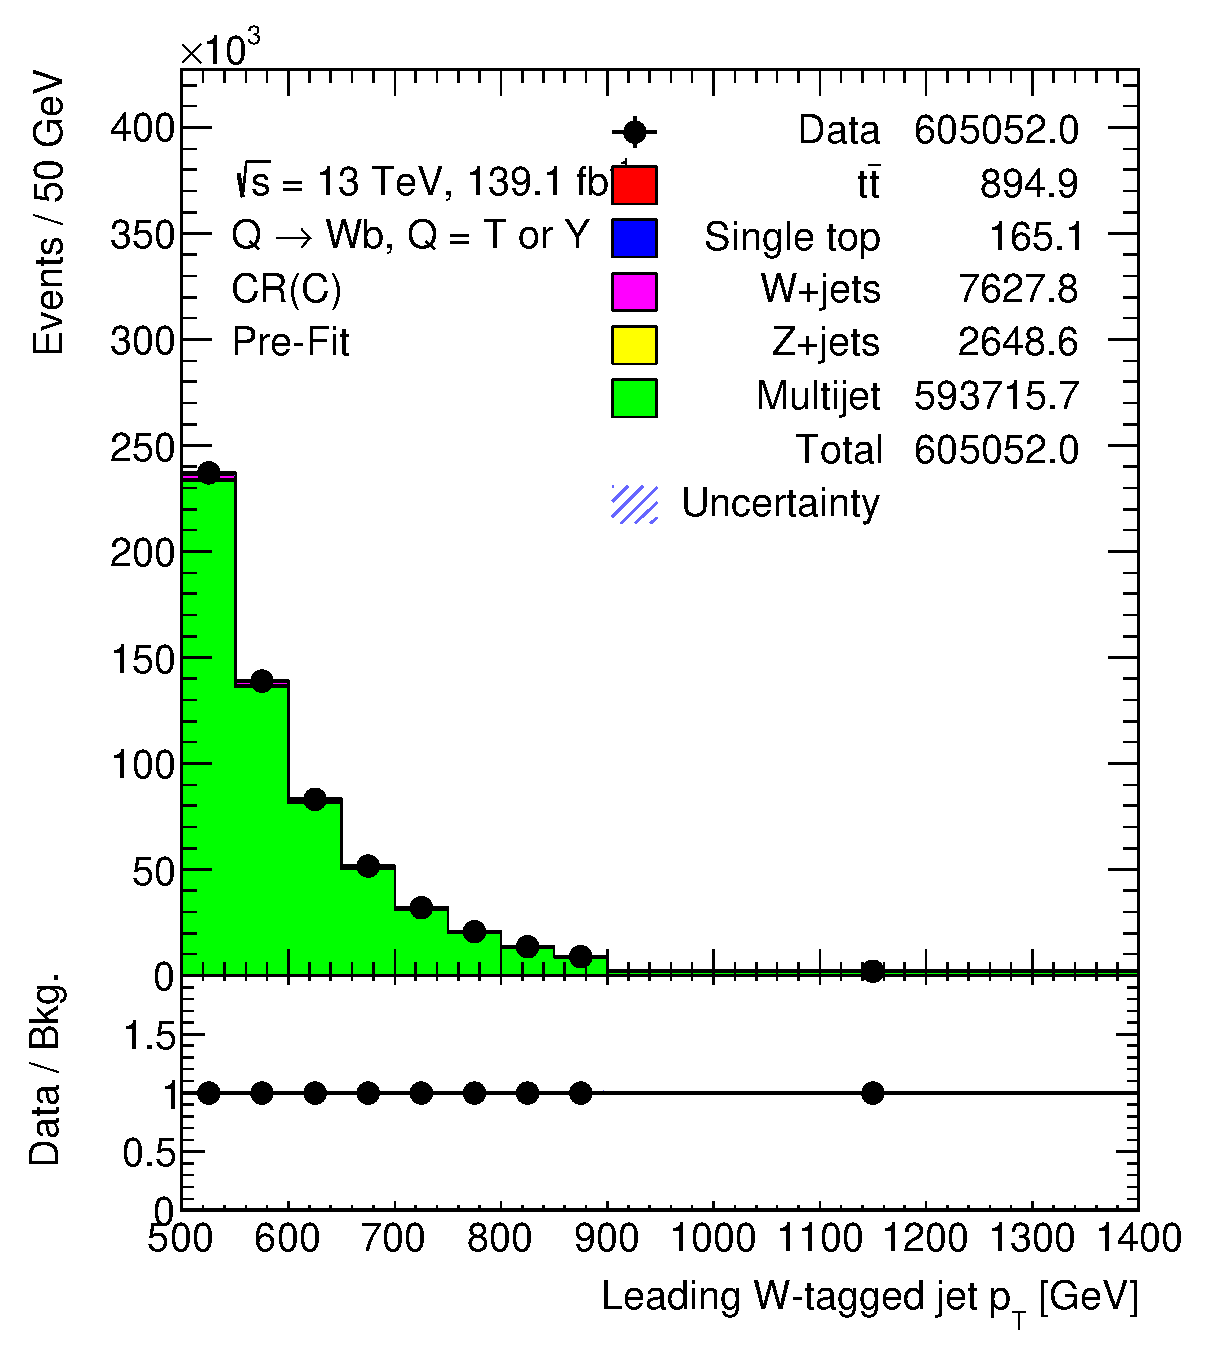
\includegraphics[width=\linewidth,height=\textheight,keepaspectratio]{CR_C_ljet_pt.eps}
		\caption{}
		\label{fig:app:cr_c:ljet_pt}
	\end{subfigure}\hspace{0.6cm}
	\begin{subfigure}{.35\textwidth}
		\centering
		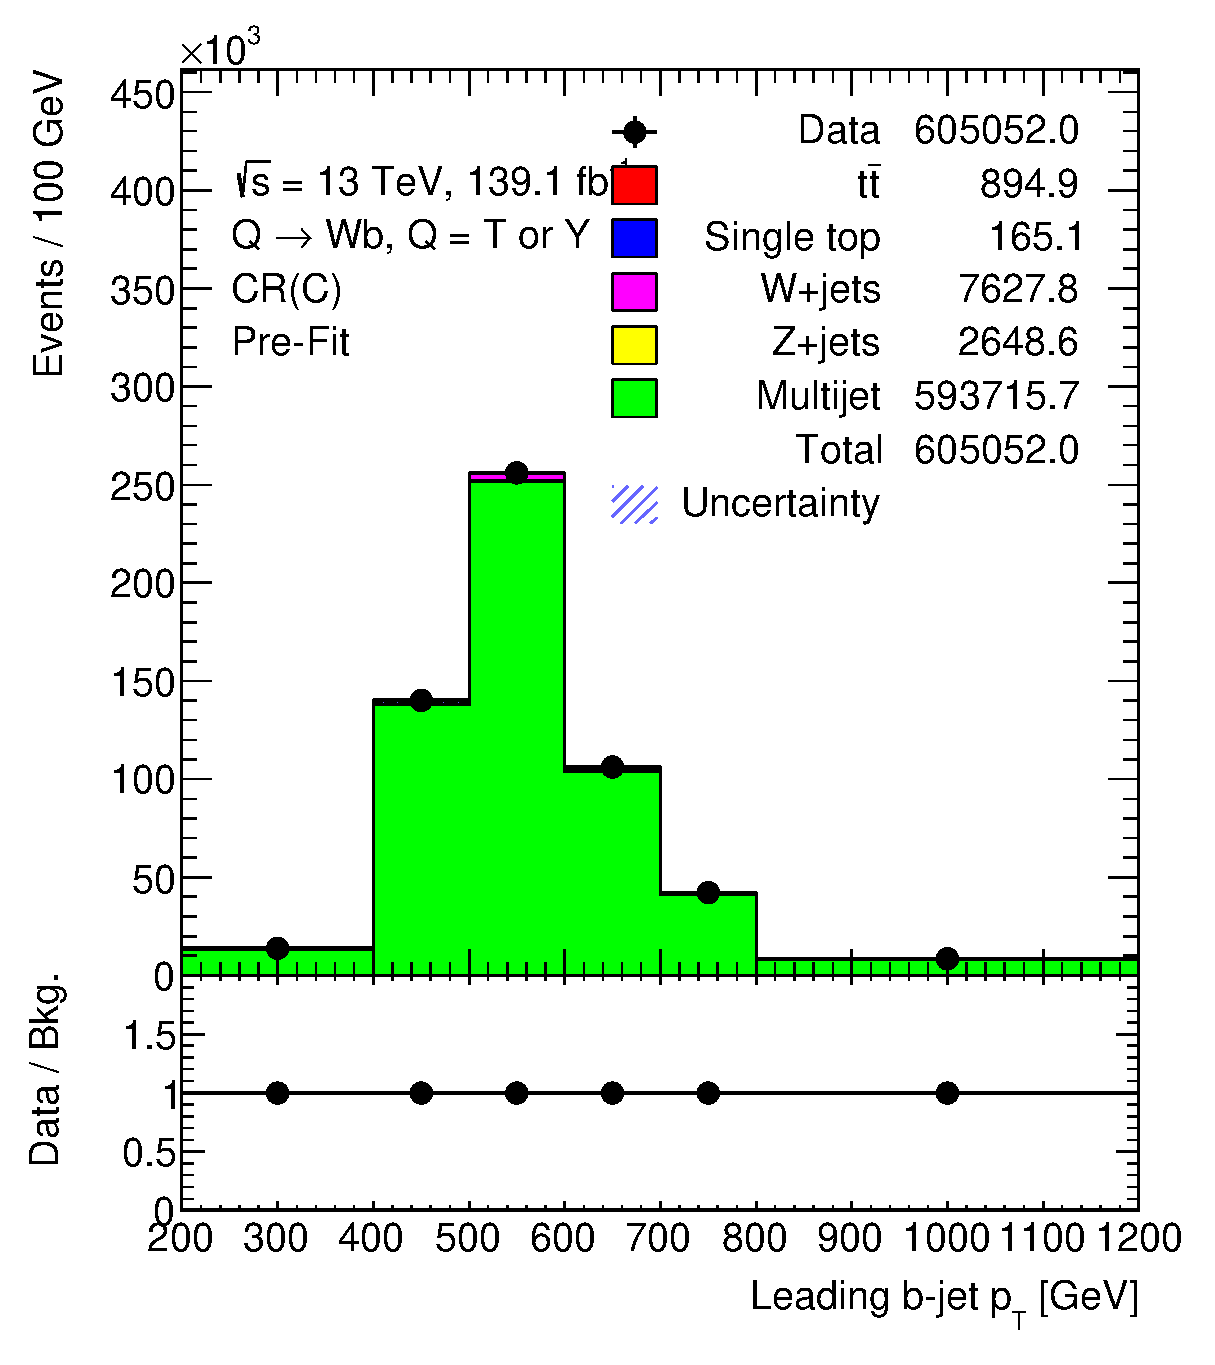
\includegraphics[width=\linewidth,height=\textheight,keepaspectratio]{CR_C_jet_pt.eps}
		\caption{}
		\label{fig:app:cr_c:jet_pt}
	\end{subfigure}
	\begin{subfigure}{.35\textwidth}
		\centering
		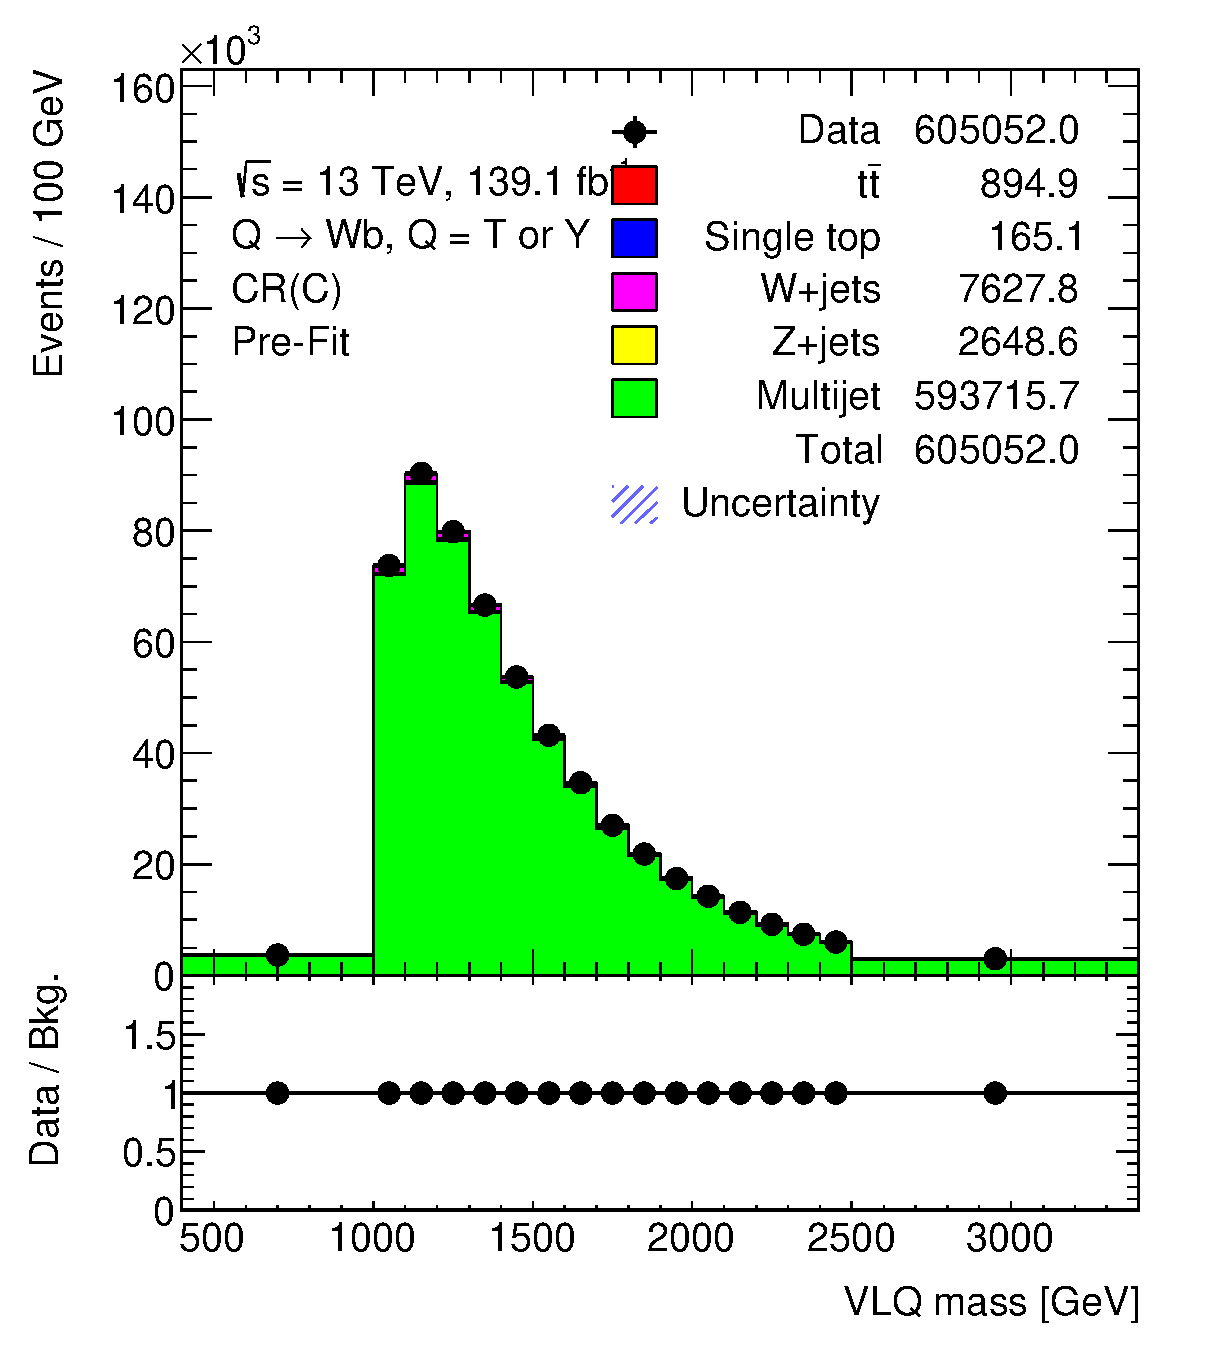
\includegraphics[width=\linewidth,height=\textheight,keepaspectratio]{CR_C_VLQM.eps}
		\caption{}
		\label{fig:app:cr_c:VLQM}
	\end{subfigure}\hspace{0.6cm}
	\begin{subfigure}{.35\textwidth}
		\centering
		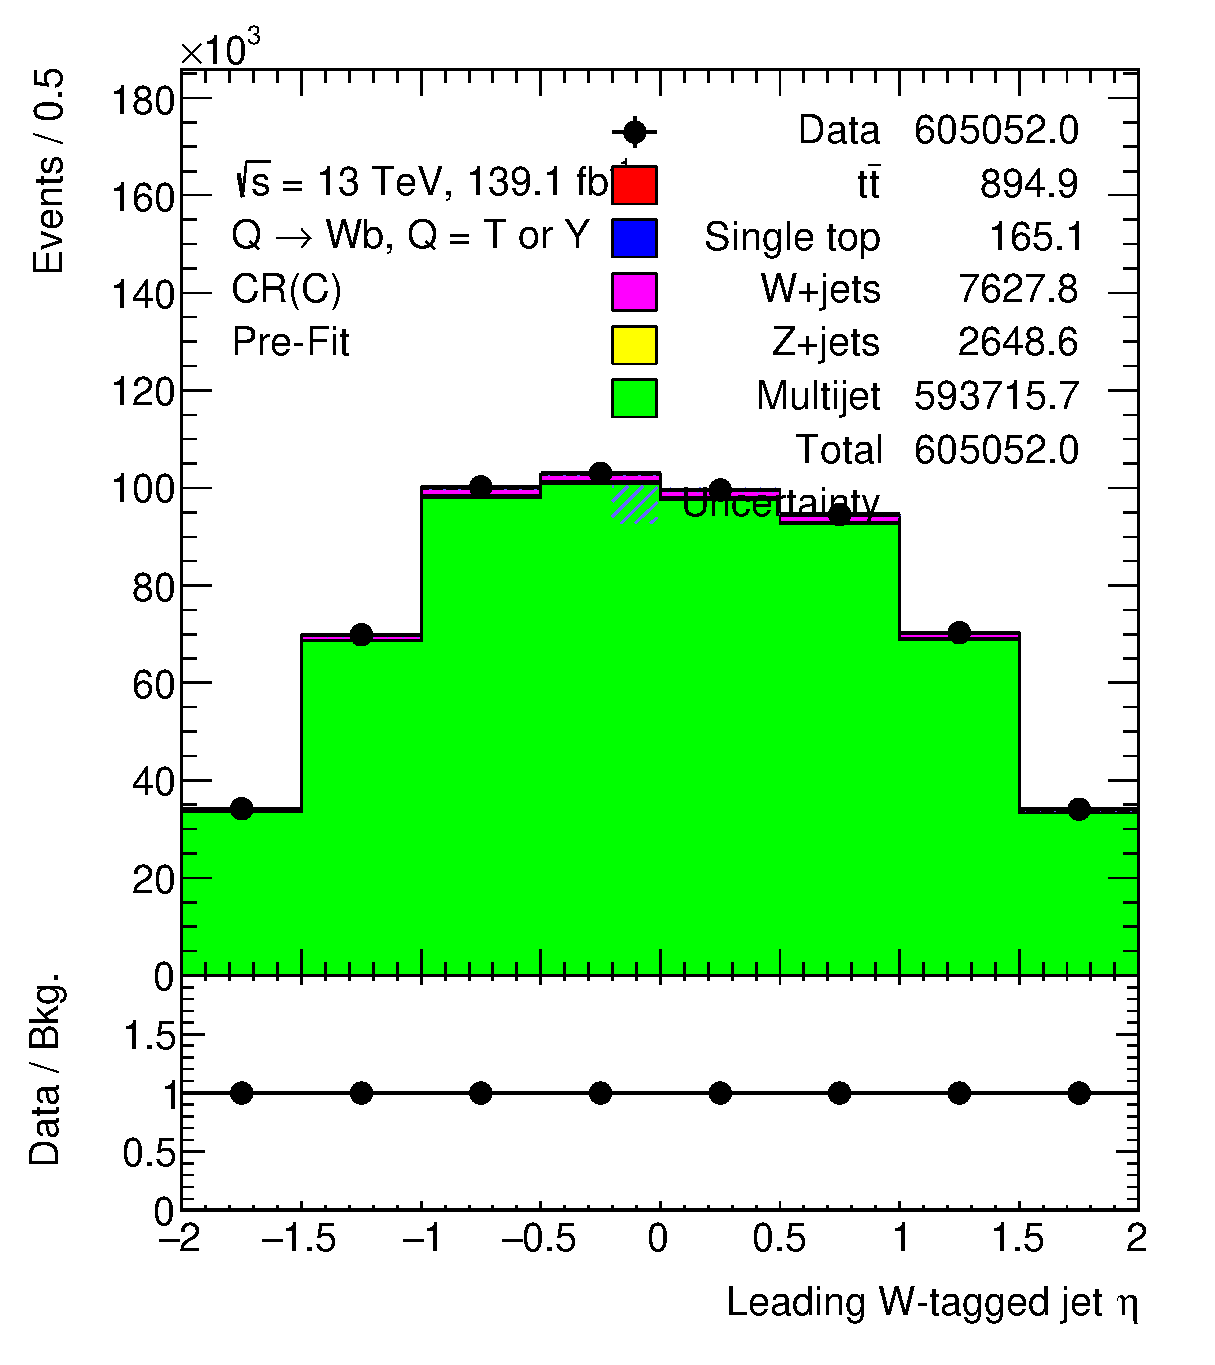
\includegraphics[width=\linewidth,height=\textheight,keepaspectratio]{CR_C_ljet_eta.eps}
		\caption{}
		\label{fig:app:cr_c:ljet_eta}
	\end{subfigure}
	\begin{subfigure}{.35\textwidth}
		\centering
		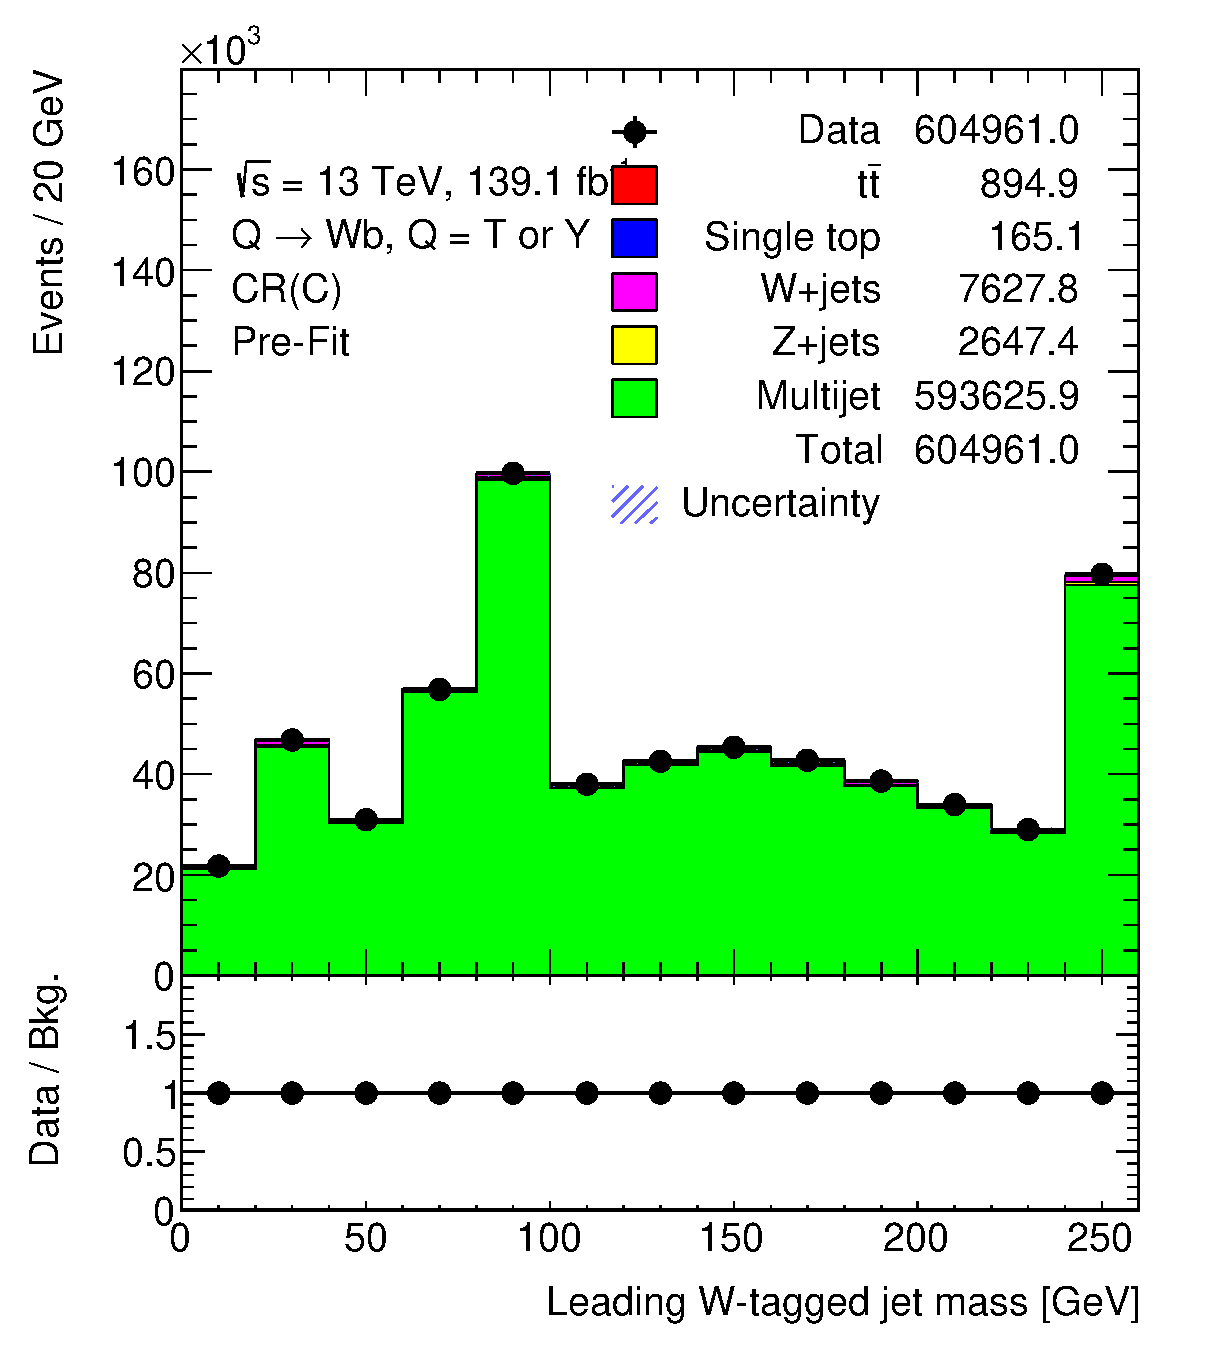
\includegraphics[width=\linewidth,height=\textheight,keepaspectratio]{CR_C_ljet_m.eps}
		\caption{}
		\label{fig:app:cr_c:ljet_m}
	\end{subfigure}\hspace{0.6cm}
	\begin{subfigure}{.35\textwidth}
		\centering
		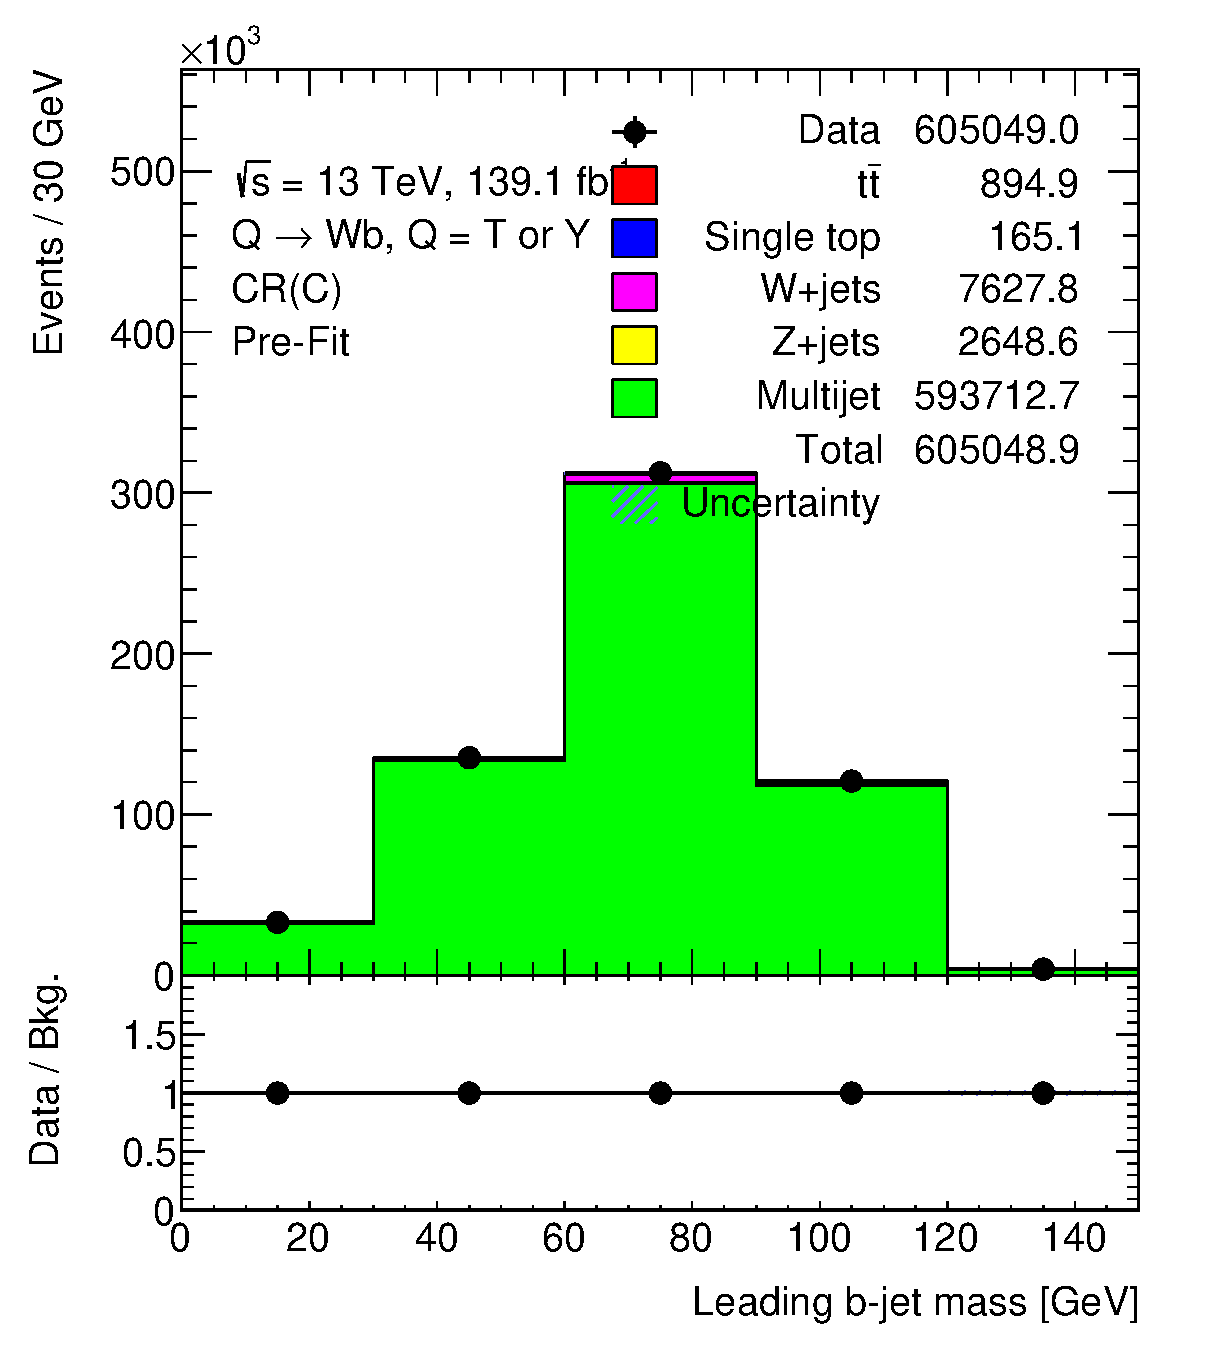
\includegraphics[width=\linewidth,height=\textheight,keepaspectratio]{CR_C_jet_m.eps}
		\caption{}
		\label{fig:app:cr_c:jet_m}
	\end{subfigure}
	\caption{A data/bkg.\ comparison of kinematic and reconstructed variables in CR C where the multijet background (in green) is calculated by Eqn.\ \ref{eqn:app} and the other backgrounds are from the MC simulation. The variables include (a) $p_{\text{T}}$ of $W$-tagged large-$R$ jet, (b) $p_{\text{T}}$ of leading $b$-tagged small-$R$ jet, (c) VLQ mass reconstructed from the kinematics of $W$-tagged large-$R$ jet and leading $b$-tagged small-$R$ jet, (d) $\eta$ distribution of $W$-tagged large-$R$ jet, (e) mass of $W$-tagged large-$R$ jet, and (f) mass of leading $b$-tagged small-$R$ jet.}
	\label{fig:app:cr_c}
\end{figure}








\begin{figure}[hbt!]
	\centering
	\graphicspath{{figs/appendix/CRD/}}
	\begin{subfigure}{.35\textwidth}
		\centering
		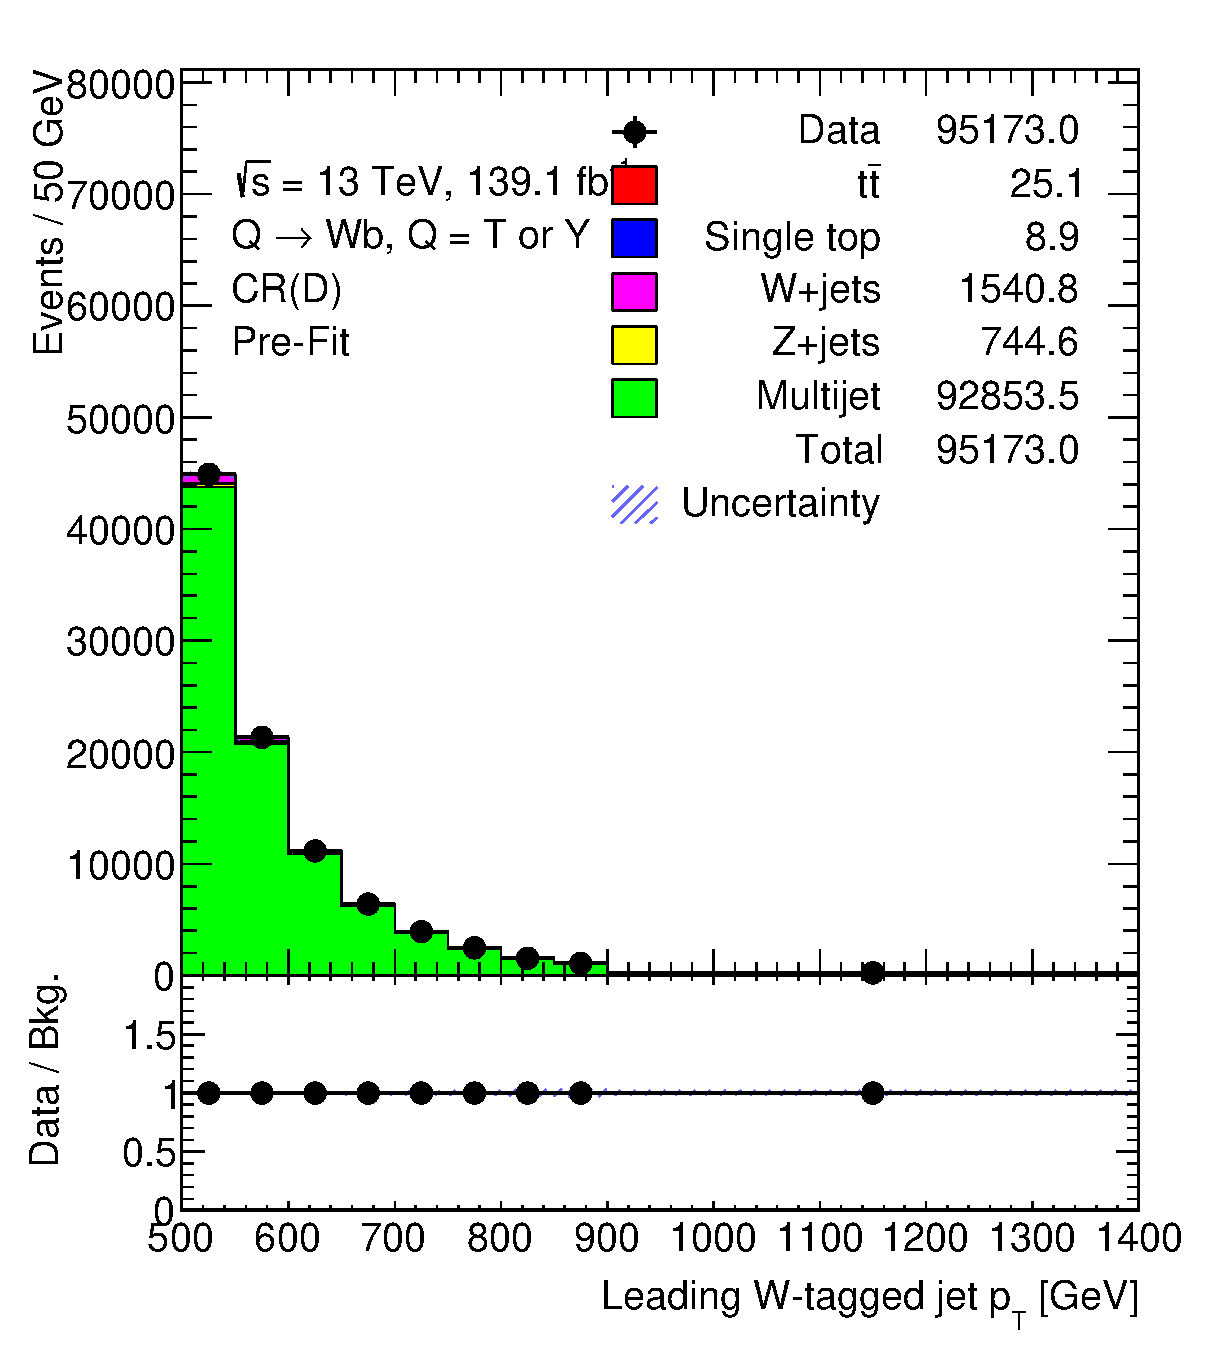
\includegraphics[width=\linewidth,height=\textheight,keepaspectratio]{CR_D_ljet_pt.eps}
		\caption{}
		\label{fig:app:cr_d:ljet_pt}
	\end{subfigure}\hspace{0.6cm}
	\begin{subfigure}{.35\textwidth}
		\centering
		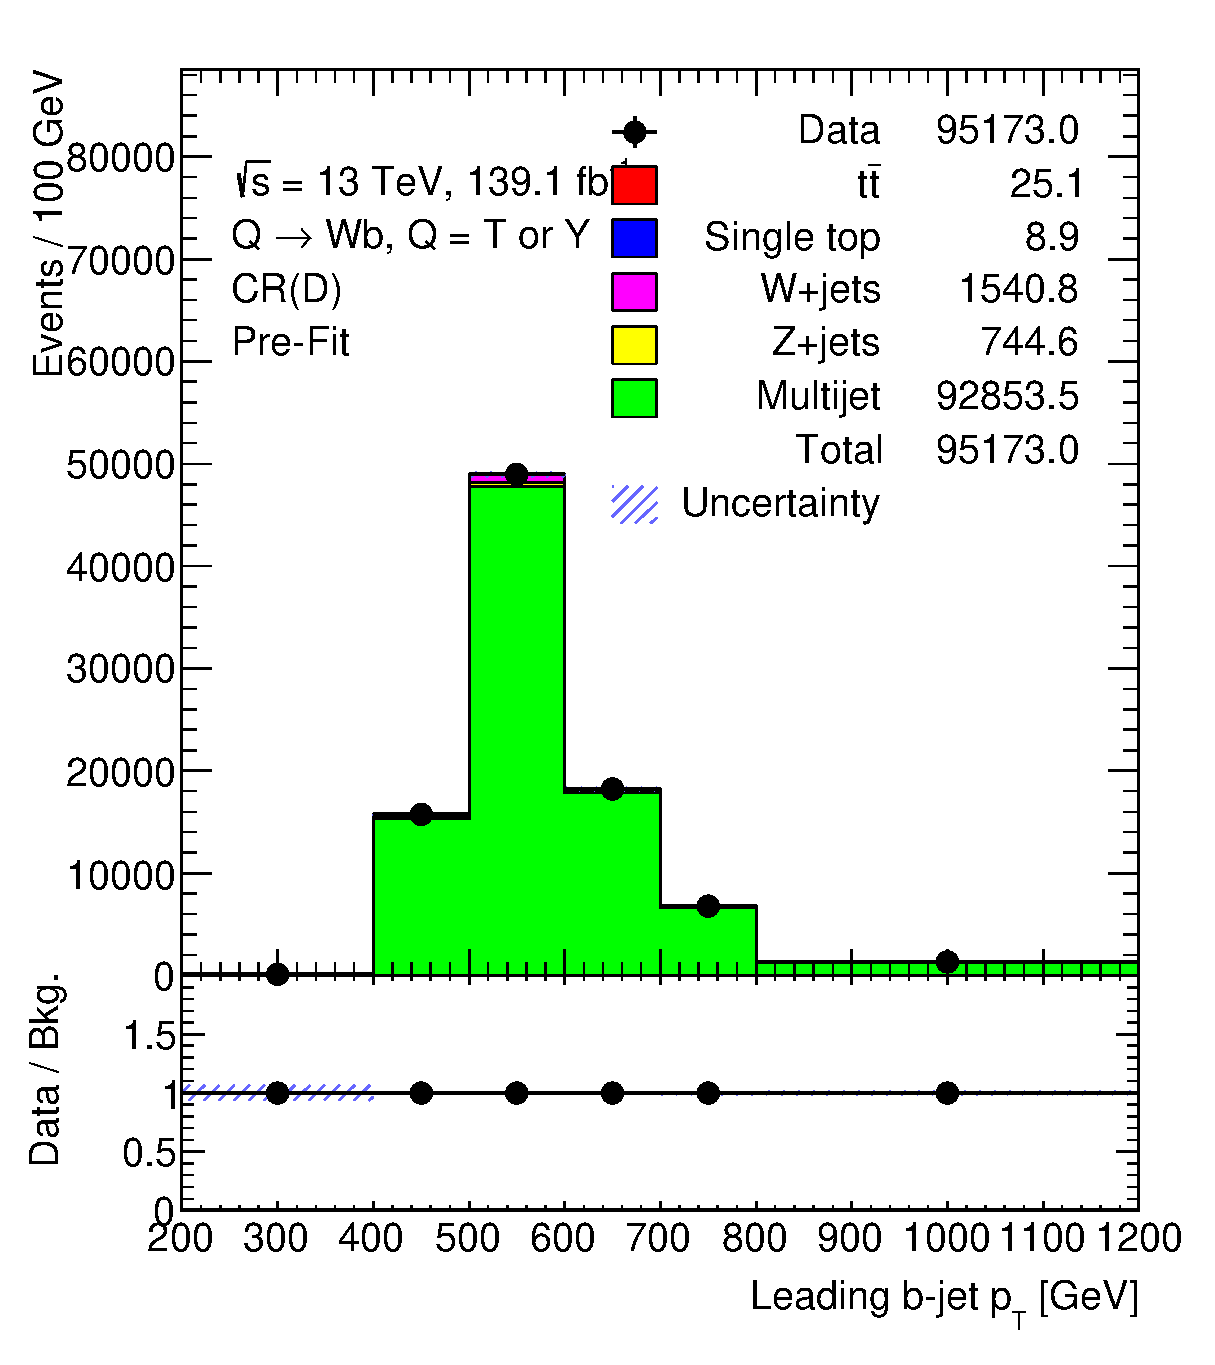
\includegraphics[width=\linewidth,height=\textheight,keepaspectratio]{CR_D_jet_pt.eps}
		\caption{}
		\label{fig:app:cr_d:jet_pt}
	\end{subfigure}
	\begin{subfigure}{.35\textwidth}
		\centering
		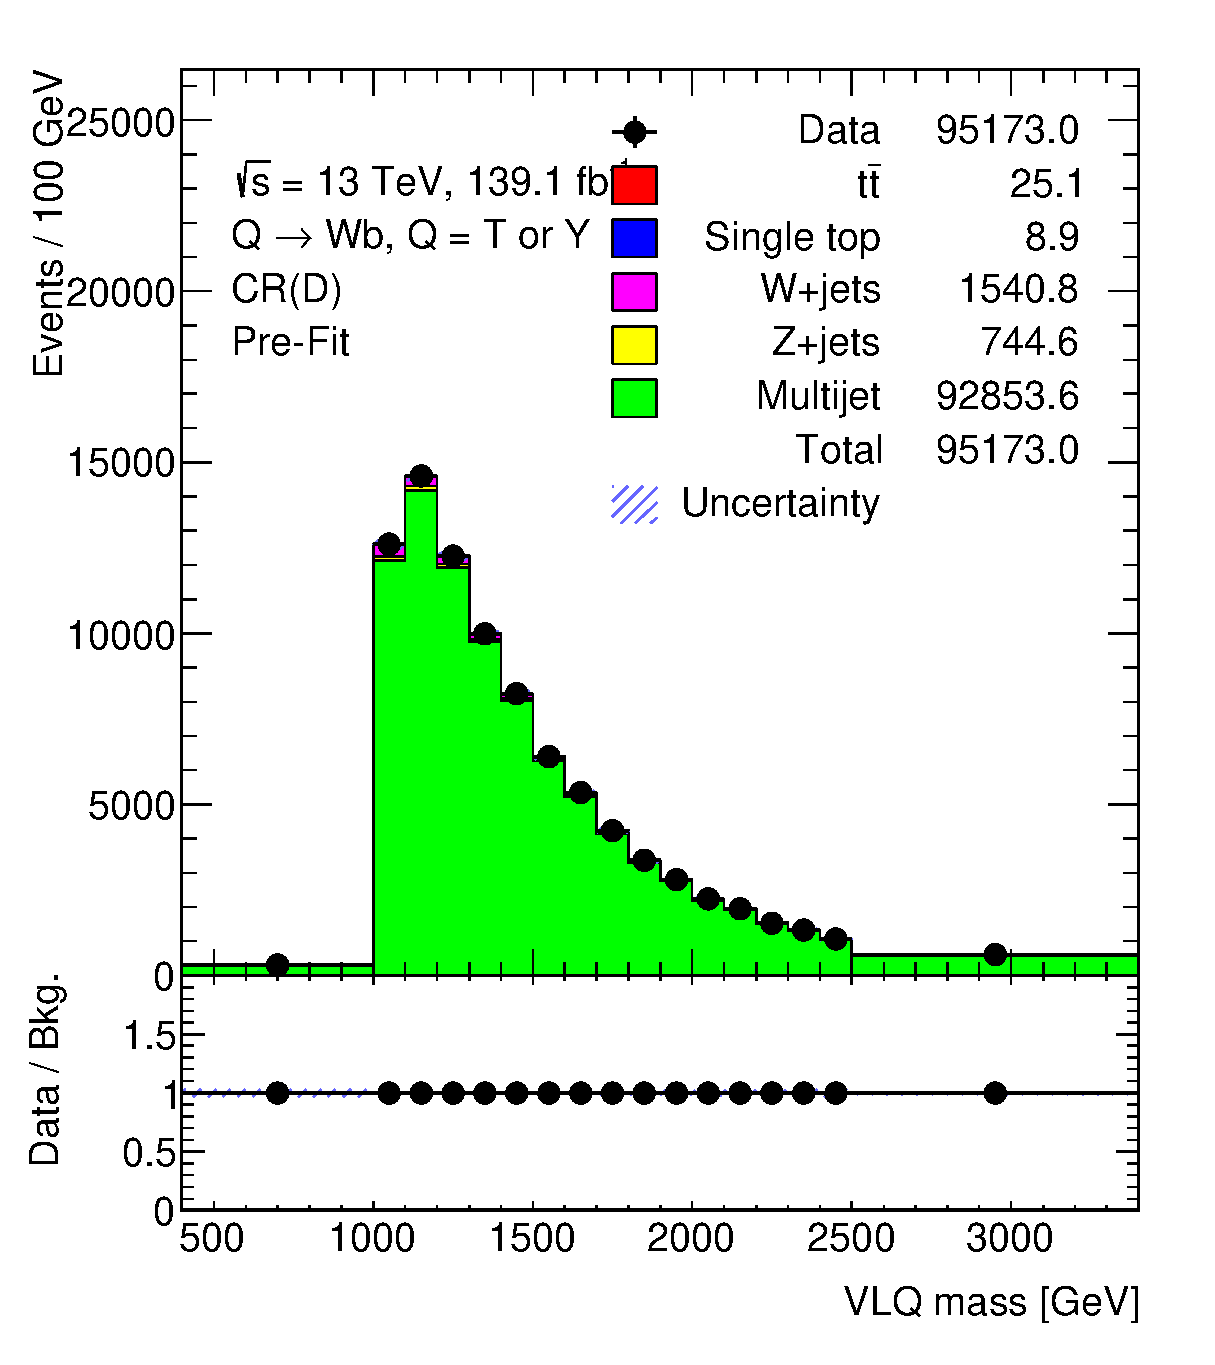
\includegraphics[width=\linewidth,height=\textheight,keepaspectratio]{CR_D_VLQM.eps}
		\caption{}
		\label{fig:app:cr_d:VLQM}
	\end{subfigure}\hspace{0.6cm}
	\begin{subfigure}{.35\textwidth}
		\centering
		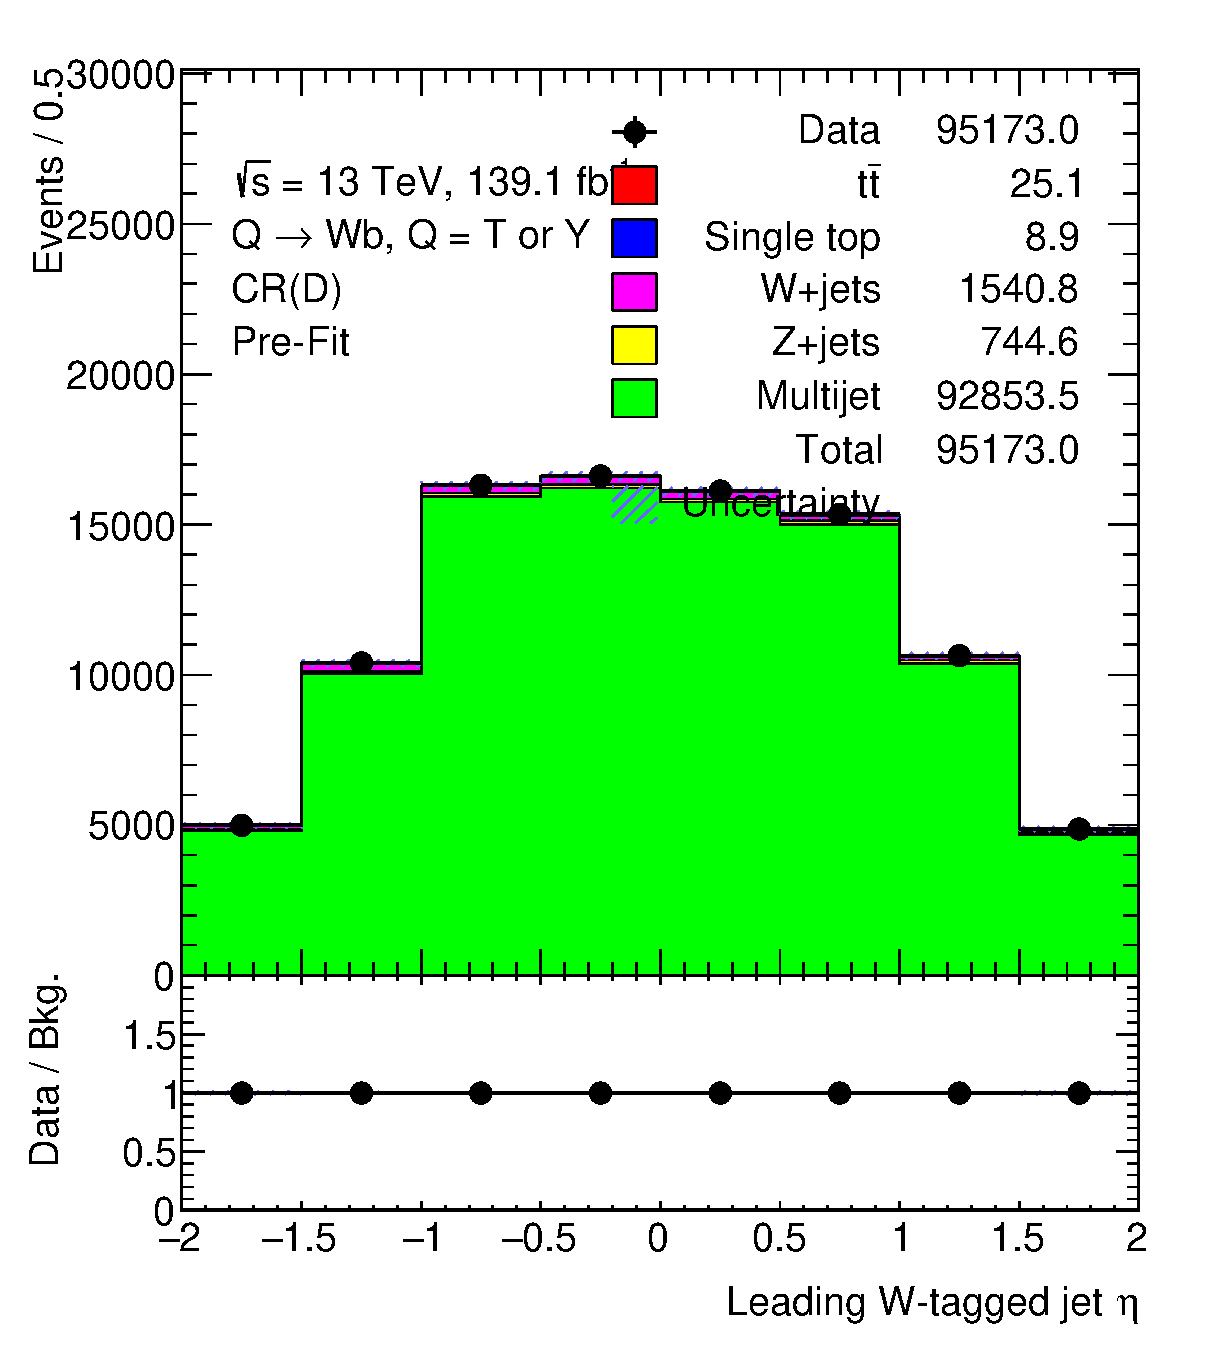
\includegraphics[width=\linewidth,height=\textheight,keepaspectratio]{CR_D_ljet_eta.eps}
		\caption{}
		\label{fig:app:cr_d:ljet_eta}
	\end{subfigure}
	\begin{subfigure}{.35\textwidth}
		\centering
		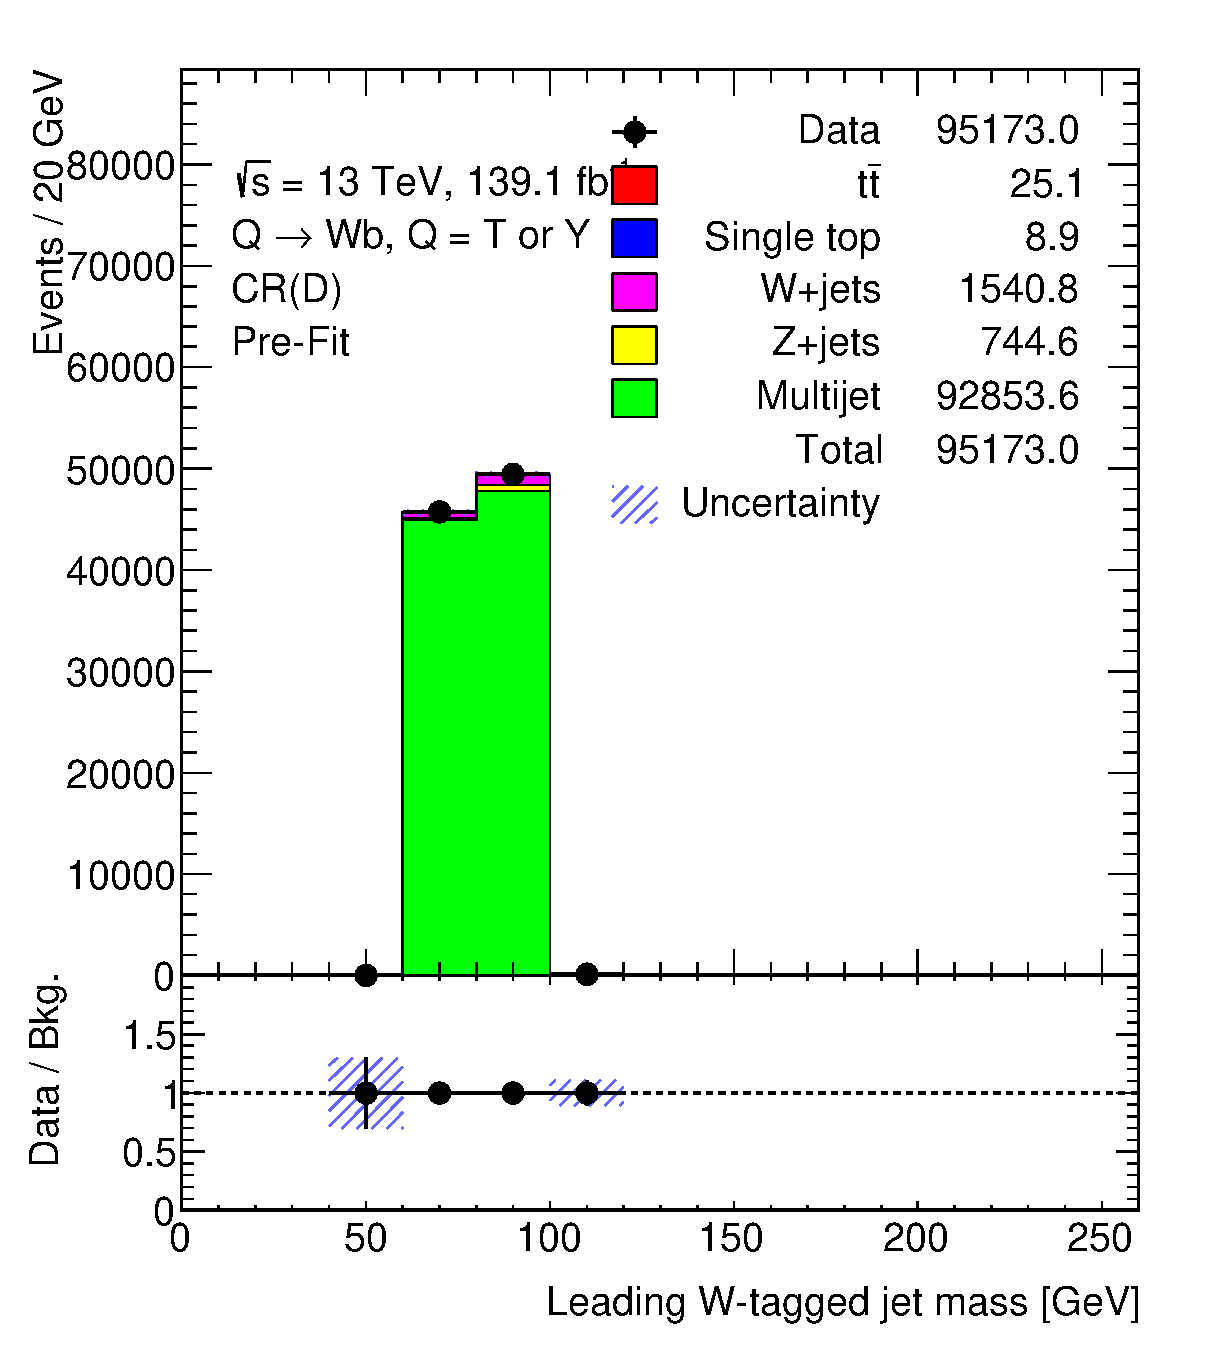
\includegraphics[width=\linewidth,height=\textheight,keepaspectratio]{CR_D_ljet_m.eps}
		\caption{}
		\label{fig:app:cr_d:ljet_m}
	\end{subfigure}\hspace{0.6cm}
	\begin{subfigure}{.35\textwidth}
		\centering
		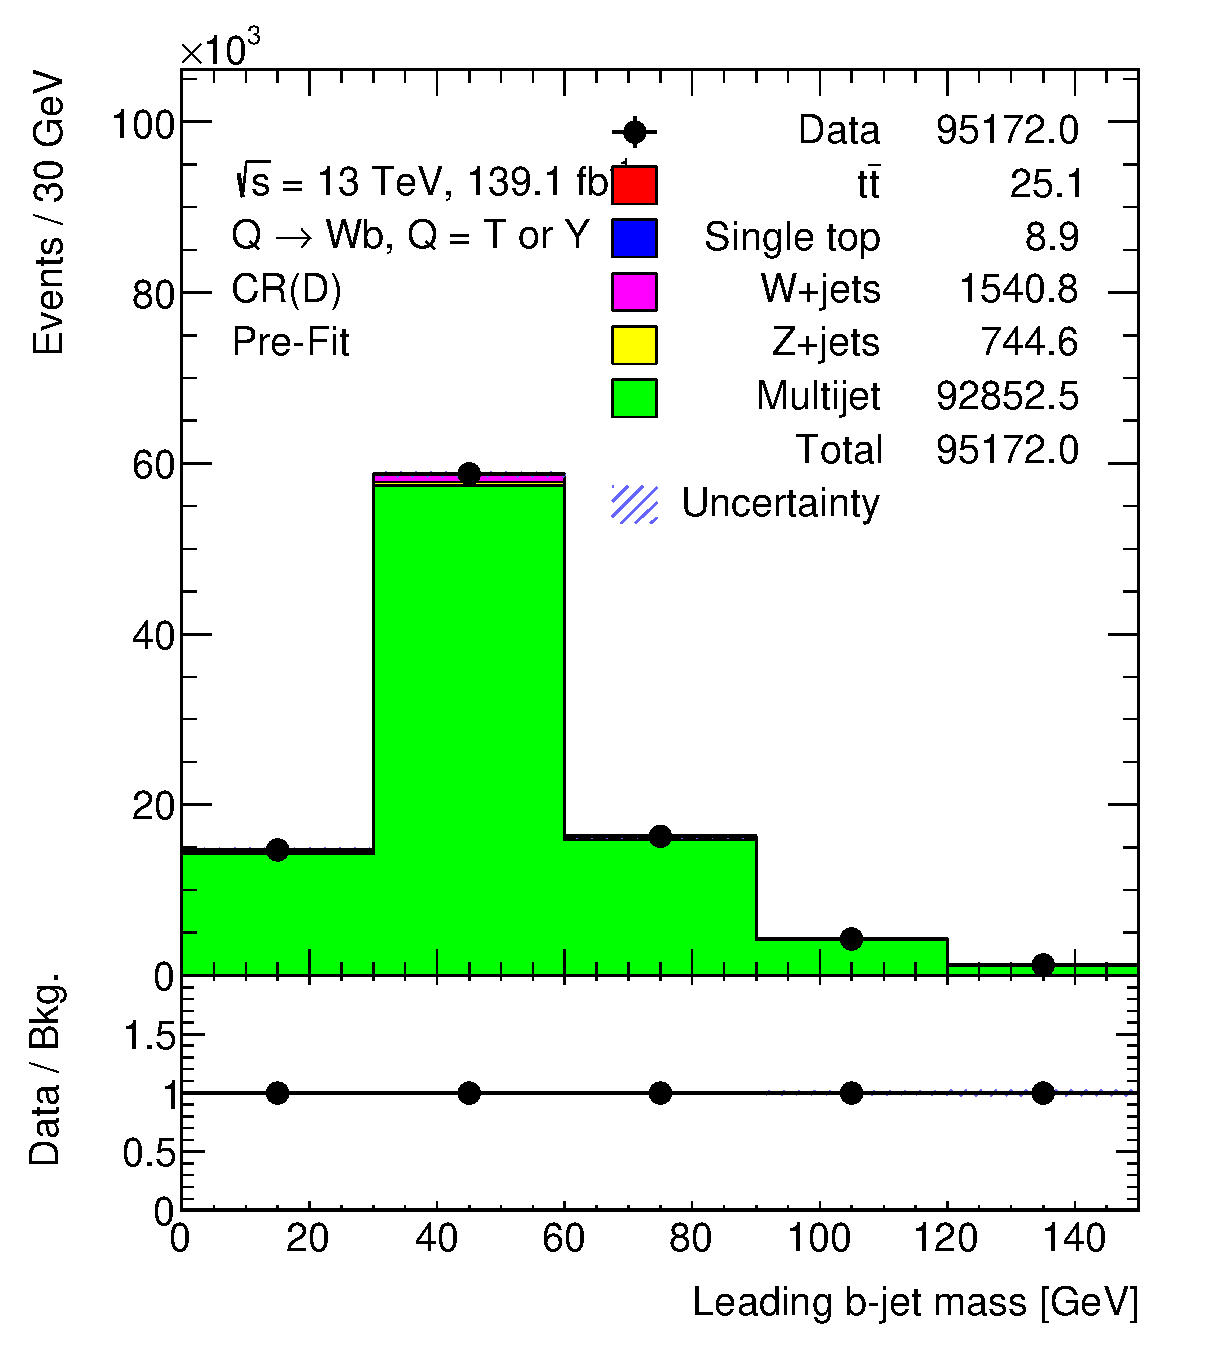
\includegraphics[width=\linewidth,height=\textheight,keepaspectratio]{CR_D_jet_m.eps}
		\caption{}
		\label{fig:app:cr_d:jet_m}
	\end{subfigure}
	\caption{A data/bkg.\ comparison of kinematic and reconstructed variables in CR D where the multijet background (in green) is calculated by Eqn.\ \ref{eqn:app} and the other backgrounds are from the MC simulation. The variables include (a) $p_{\text{T}}$ of $W$-tagged large-$R$ jet, (b) $p_{\text{T}}$ of leading $b$-tagged small-$R$ jet, (c) VLQ mass reconstructed from the kinematics of $W$-tagged large-$R$ jet and leading $b$-tagged small-$R$ jet, (d) $\eta$ distribution of $W$-tagged large-$R$ jet, (e) mass of $W$-tagged large-$R$ jet, and (f) mass of leading $b$-tagged small-$R$ jet.}
	\label{fig:app:cr_d}
\end{figure}





\begin{figure}[hbt!]
	\centering
	\graphicspath{{figs/appendix/CRD1/}}
	\begin{subfigure}{.35\textwidth}
		\centering
		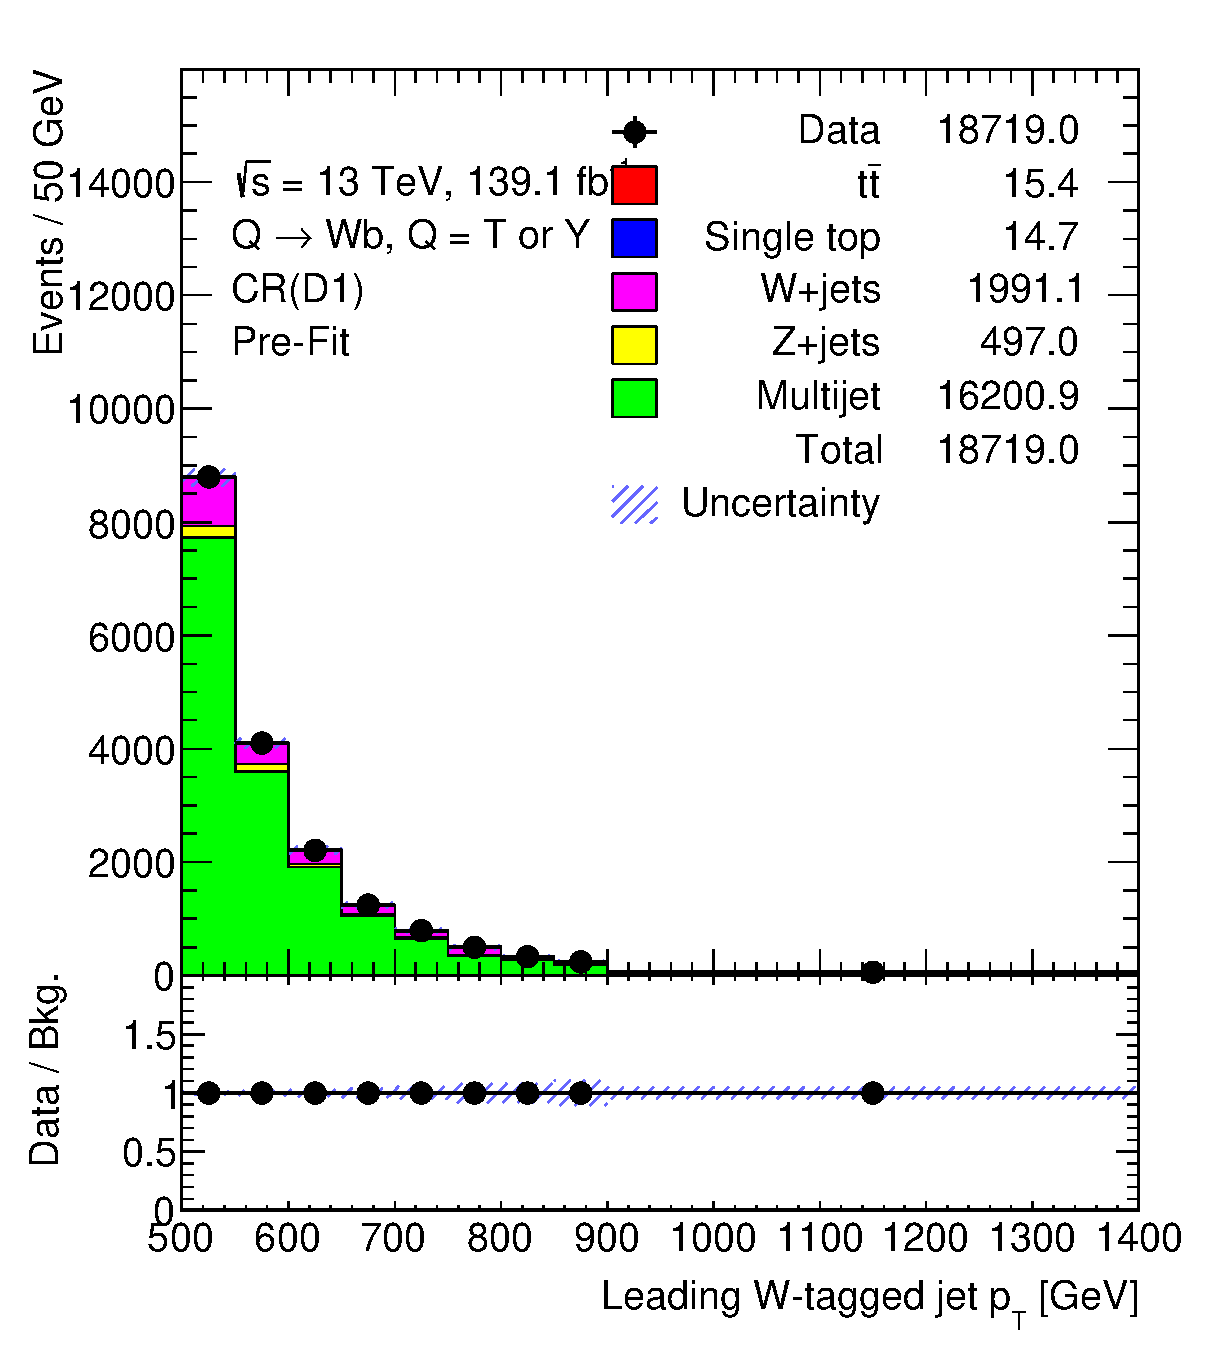
\includegraphics[width=\linewidth,height=\textheight,keepaspectratio]{CR_D1_ljet_pt.eps}
		\caption{}
		\label{fig:app:cr_d1:ljet_pt}
	\end{subfigure}\hspace{0.6cm}
	\begin{subfigure}{.35\textwidth}
		\centering
		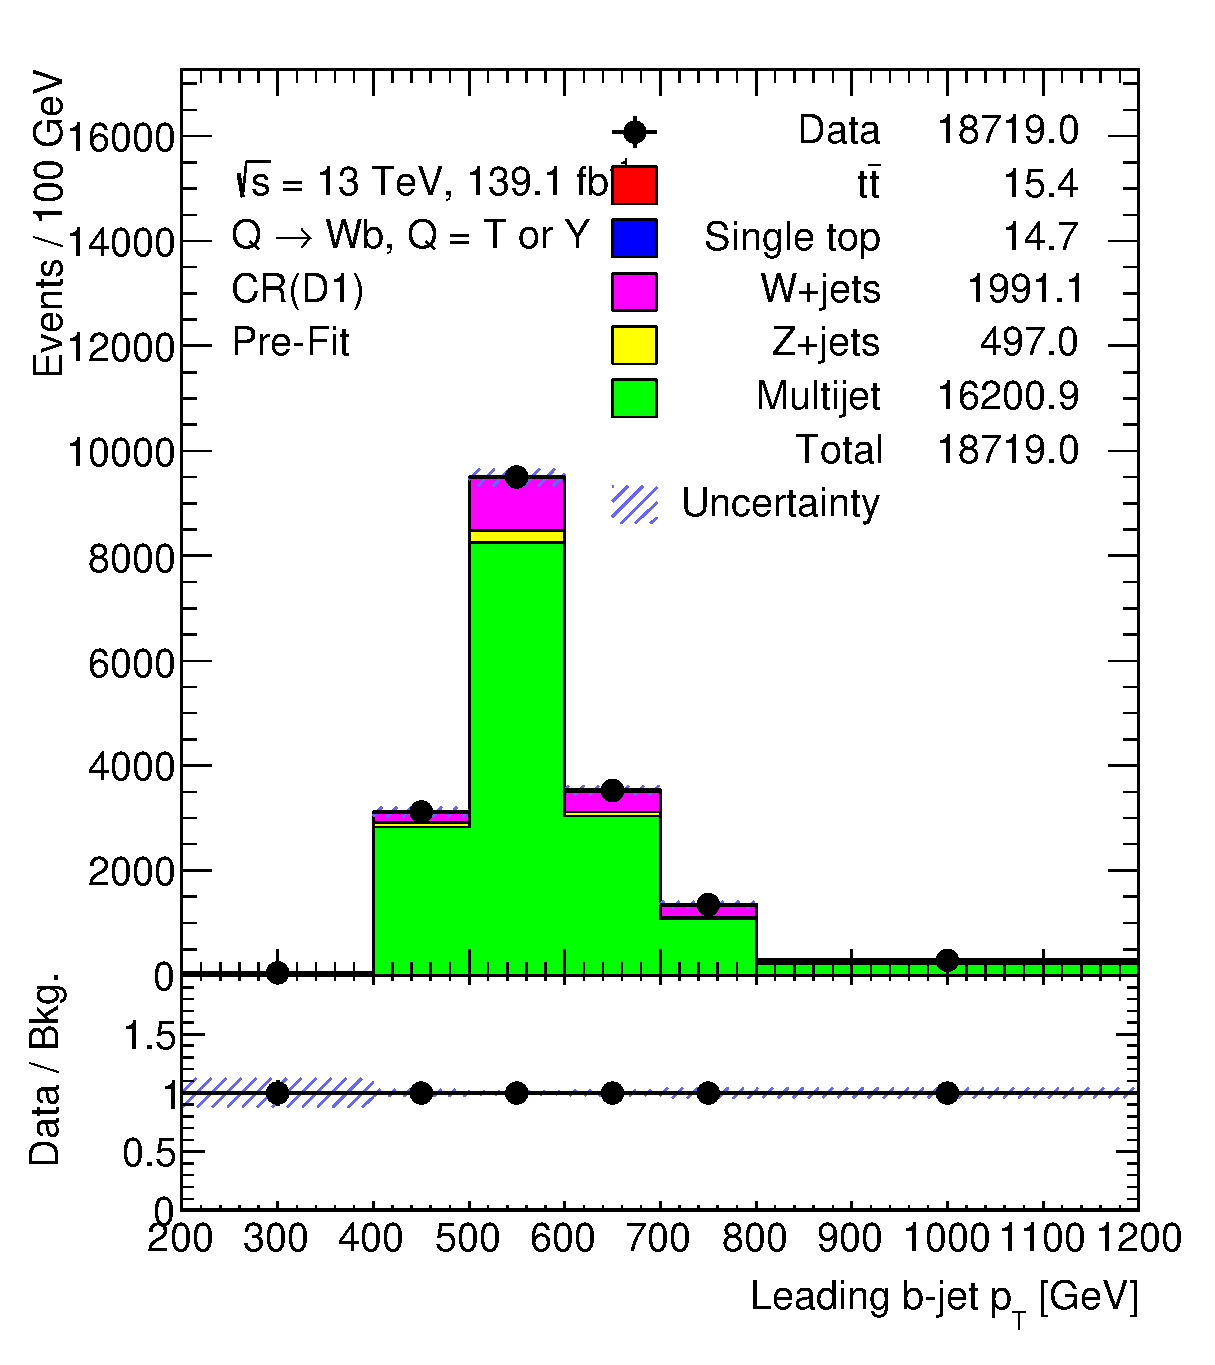
\includegraphics[width=\linewidth,height=\textheight,keepaspectratio]{CR_D1_jet_pt.eps}
		\caption{}
		\label{fig:app:cr_d1:jet_pt}
	\end{subfigure}
	\begin{subfigure}{.35\textwidth}
		\centering
		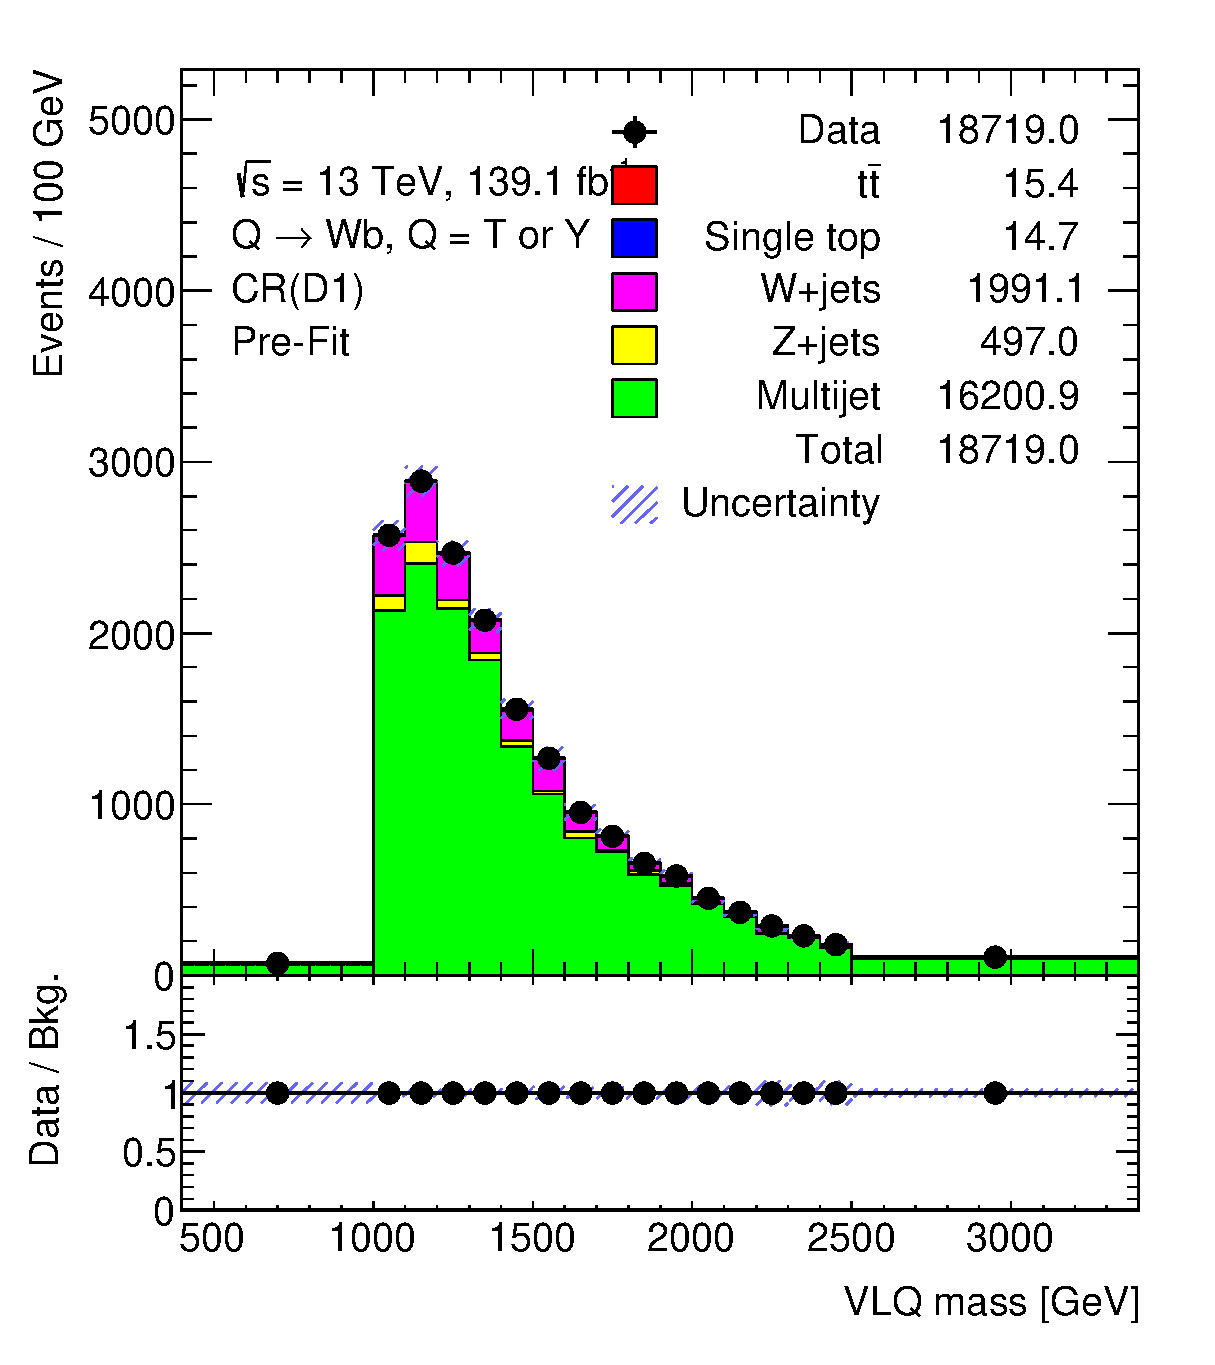
\includegraphics[width=\linewidth,height=\textheight,keepaspectratio]{CR_D1_VLQM.eps}
		\caption{}
		\label{fig:app:cr_d1:VLQM}
	\end{subfigure}\hspace{0.6cm}
	\begin{subfigure}{.35\textwidth}
		\centering
		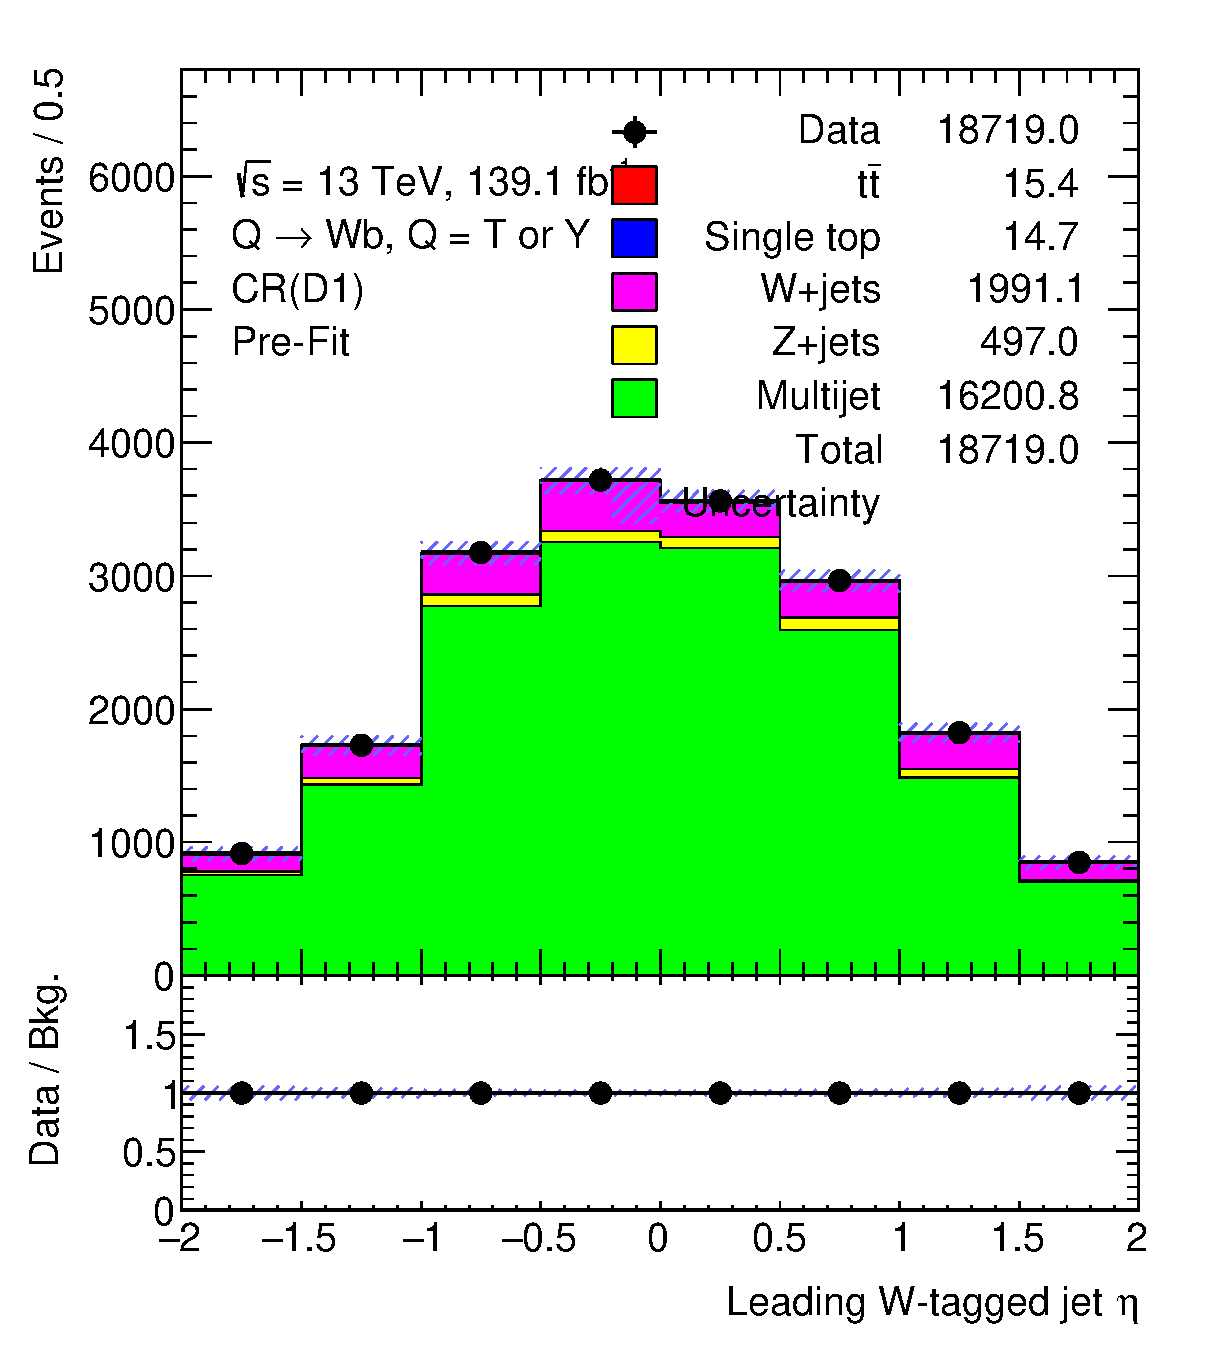
\includegraphics[width=\linewidth,height=\textheight,keepaspectratio]{CR_D1_ljet_eta.eps}
		\caption{}
		\label{fig:app:cr_d1:ljet_eta}
	\end{subfigure}
	\begin{subfigure}{.35\textwidth}
		\centering
		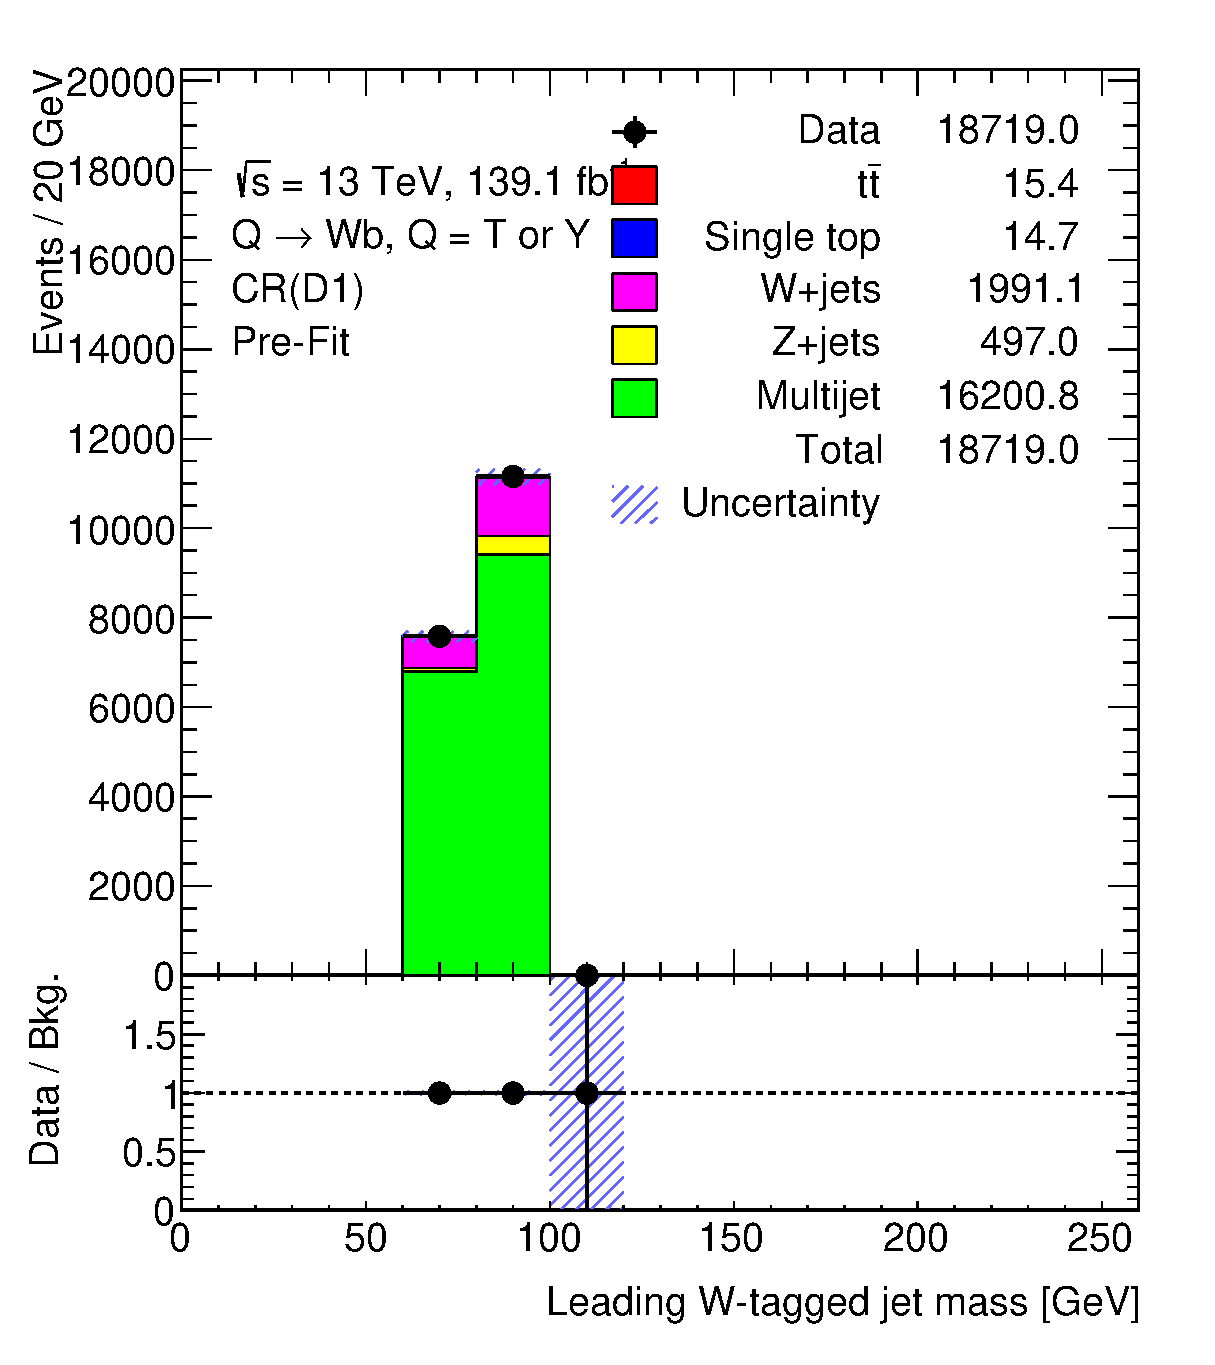
\includegraphics[width=\linewidth,height=\textheight,keepaspectratio]{CR_D1_ljet_m.eps}
		\caption{}
		\label{fig:app:cr_d1:ljet_m}
	\end{subfigure}\hspace{0.6cm}
	\begin{subfigure}{.35\textwidth}
		\centering
		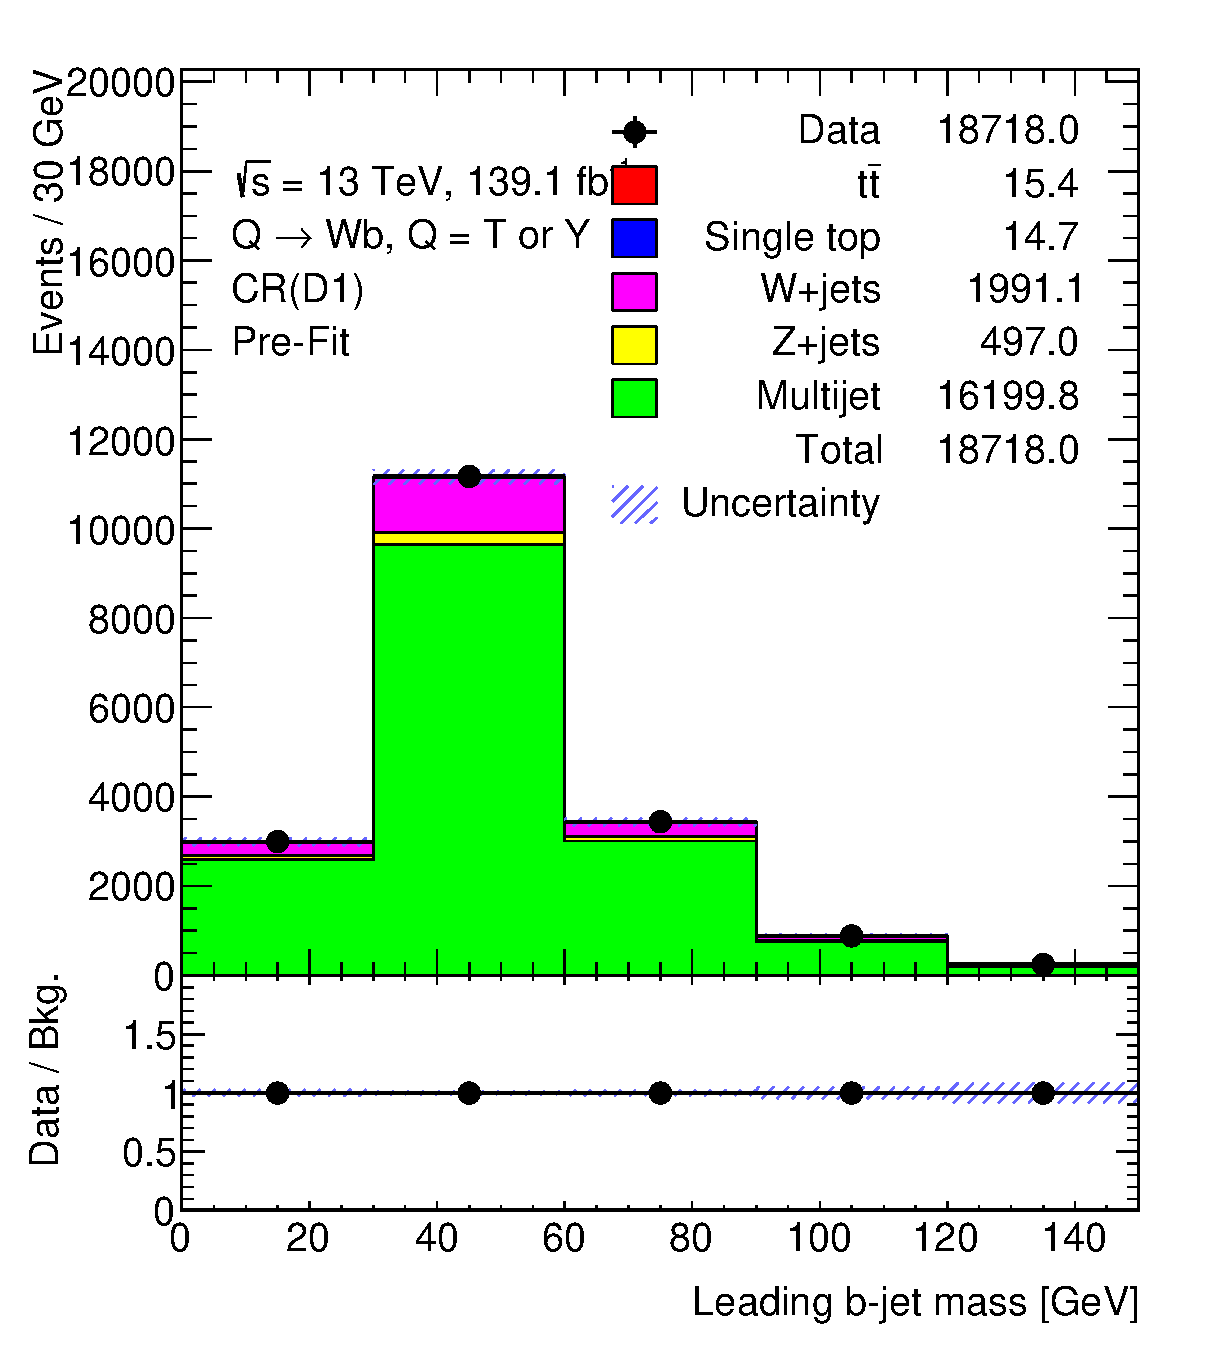
\includegraphics[width=\linewidth,height=\textheight,keepaspectratio]{CR_D1_jet_m.eps}
		\caption{}
		\label{fig:app:cr_d1:jet_m}
	\end{subfigure}
	\caption{A data/bkg.\ comparison of kinematic and reconstructed variables in CR D1 where the multijet background (in green) is calculated by Eqn.\ \ref{eqn:app} and the other backgrounds are from the MC simulation. The variables include (a) $p_{\text{T}}$ of $W$-tagged large-$R$ jet, (b) $p_{\text{T}}$ of leading $b$-tagged small-$R$ jet, (c) VLQ mass reconstructed from the kinematics of $W$-tagged large-$R$ jet and leading $b$-tagged small-$R$ jet, (d) $\eta$ distribution of $W$-tagged large-$R$ jet, (e) mass of $W$-tagged large-$R$ jet, and (f) mass of leading $b$-tagged small-$R$ jet.}
	\label{fig:app:cr_d1}
\end{figure}

%%% Local Variables: 
%%% mode: latex
%%% TeX-master: "../mythesis"
%%% End: 
